\documentclass[a4paper,12pt, oneside]{book}

%\usepackage{fullpage}
\usepackage[T1]{fontenc}
\usepackage[italian]{babel}
\usepackage[utf8]{inputenc}
\usepackage{amssymb}
\usepackage{amsthm}
\usepackage{graphics}
\usepackage{amsfonts}
\usepackage{listings}
\usepackage{amsmath}
\usepackage{amstext}
\usepackage{engrec}
\usepackage{rotating}
\usepackage[safe,extra]{tipa}
\usepackage{showkeys}
\usepackage{multirow}
\usepackage{hyperref}
\usepackage{microtype}
\usepackage{enumerate}
\usepackage{braket}
\usepackage{marginnote}
\usepackage{pgfplots}
\usepackage{cancel}
\usepackage{polynom}
\usepackage{booktabs}
\usepackage{enumitem}
\usepackage{framed}
\usepackage{pdfpages}
\usepackage{pgfplots}
\usepackage[cache=false]{minted}
 \usepackage[usenames,dvipsnames, pdf]{pstricks}
 \usepackage{epsfig}
 \usepackage{pst-grad} % For gradients
 \usepackage{pst-plot} % For axes
 \usepackage[space]{grffile} % For spaces in paths
 \usepackage{etoolbox} % For spaces in paths
 \makeatletter % For spaces in paths
 \patchcmd\Gread@eps{\@inputcheck#1 }{\@inputcheck"#1"\relax}{}{}
 \makeatother
\usepackage{fancyhdr}
\pagestyle{fancy}
\fancyhead[LE,RO]{\slshape \rightmark}
\fancyhead[LO,RE]{\slshape \leftmark}
\fancyfoot[C]{\thepage}



\title{Analisi e Progettazione del Software}
\author{UniShare\\\\Davide Cozzi\\\href{https://t.me/dlcgold}{@dlcgold}\\\\Gabriele De Rosa\\\href{https://t.me/derogab}{@derogab} \\\\Federica Di Lauro\\\href{https://t.me/f_dila}{@f\textunderscore dila}}
\date{}

\pgfplotsset{compat=1.13}
\begin{document}
\maketitle

\definecolor{shadecolor}{gray}{0.80}

\newtheorem{teorema}{Teorema}
\newtheorem{definizione}{Definizione}
\newtheorem{esempio}{Esempio}
\newtheorem{corollario}{Corollario}
\newtheorem{lemma}{Lemma}
\newtheorem{osservazione}{Osservazione}
\newtheorem{nota}{Nota}
\newtheorem{esercizio}{Esercizio}
\tableofcontents
\renewcommand{\chaptermark}[1]{%
	\markboth{\chaptername
		\ \thechapter.\ #1}{}}
\renewcommand{\sectionmark}[1]{\markright{\thesection.\ #1}}
\chapter{Introduzione}
\textbf{Questi appunti sono presi durante le lezioni in aula. Per quanto sia stata fatta una revisione è altamente probabile (praticamente certo) che possano contenere errori, sia di stampa che di vero e proprio contenuto. Per eventuali proposte di correzione effettuare una pull request. Link: } \url{https://github.com/dlcgold/Appunti}.\\
\textbf{Grazie mille e buono studio!}
\chapter{Introduzione all'Ingegneria del software}
Durante il corso di Analisi e Progettazione del software si analizzano i modelli e i principi per lo sviluppo di un
software mantenibile, andando anche ad analizzare, in maniera sommaria, anche tutti gli strumenti di
ingegneria del software, necessari per lo sviluppo ottimale di un software.

In questo corso studieremo in dettaglio i seguenti argomenti:
\begin{itemize}
	\item introduzione all'ingegneria del software
	\item progettazione sistemi orientati ad oggetti
	\item modellazione a dominio
	\item UML e analisi dei casi d'uso
	\item design pattern
	\item sviluppo test-driven(cenni)
	\item code smell e refactoring(cenni)
\end{itemize}
Il software, è l'insieme delle componenti modificabili e non fisiche di un calcolatore, viene diviso in due categorie:
\begin{description}
	\item [generici], per un ampio range di clienti, come ad esempio gli elaboratori di testi
	\item [custom], per un singolo cliente, come ad esempio i gestionali specifici di un impresa
\end{description}
Questa differenza si sta sempre più assottiliando in quanto recentemente varie aziende stanno sviluppando un
software generico, che viene poi adattato in base alle esigenze del singolo cliente,
come ad esempio i software Oracle e Sas.

Nello sviluppo di software si utlizza spesso una base pre-esistente, infatti l'ingegneria del software si occupa
di tutti gli aspetti per lo sviluppo del software, sfruttando di solito una base preesistente. \newline
Di solito quando si sviluppa un software si presuppone che abbia una durata di alcuni anni, con la predispozione
al cambiamento e all'introduzione di nuove features infatti un software per essere utile deve essere continuamente cambiato.

Si hanno due tipologie di progetti:
\begin{enumerate}
	\item \textbf{progetti di routine}, con soluzione di problemi e riuso di vecchio codice
	\item \textbf{progetti innovativi}, con soluzioni nuovi
\end{enumerate}
e solitamente l'ingegneria del software si occupa principalmente di progetti innovativi
con specifiche del progetto variabili, con la presenza di cambiamenti continui e ovviamente
non è uguale nè similare con l'ingegneria tradizionale.

Un programmatore normalmente lavora da solo, su un programma completo con specifiche note mentre un ingegnere del software
lavora in gruppo, progetta componenti e l'architettura e identifica requisiti e specifiche.
Il costo del software spesso supera quello hardware %aggiungere grafico

Nello sviluppo di un software si hanno le seguenti fasi di sviluppo:
\begin{itemize}
	\item \textbf{analisi dei requisiti}, che indica cosa deve fare il sistema
	\item \textbf{progettazione}, progetto del sistema d implementare
	\item \textbf{sviluppo}, produzione del sistema software
	\item \textbf{convalida}, verifica dei requisiti del cliente
	\item \textbf{evoluzione}, evoluzione al cambiare di requisiti del cliente
\end{itemize}
Esistono dei sistemi software per l'automazione delle attività svolte nel progetto software,
i cosiddetti \textbf{CASE} (Computer-Aided Software Engineering) che si dividono in:
\begin{description}
	\item [CASE di alto livello] per il supporto alle prime attività di processo come la raccolta requisiti e la progettazione
	\item [CASE di basso livello] per il supporto alle ultime attività di processo come la programmazione,
	      il debugging, testing e reverse engineering
\end{description}
Nella figure X1 e X2  si hanno delle risposte alle comuni domande sull'ingegneria del software e le caratteristiche
di un ottimo software, necessario per mantenerlo facilmente modificabile nel tempo.

Nello sviluppo di un software, qualsiasi tipologia esso sia, prevede i seguenti aspetti in comune:
\begin{description}
	\item [specifiche del software] vengono definite le specifiche e analizzato in dettaglio il comportamento
	      e le funzionalità richieste da sviluppare
	\item [sviluppo del software] viene effettivamente implementato e progettato il codice, attraverso i tools di sviluppo,
	      rispettando le specifiche previste nella fase precedente.
	\item [convalida del software] viene testato il software sviluppato nella fase precedente, al f
	\item [evoluzione del software] viene mantenuto ed evoluto il software, al fine di riflettere i cambiamenti e delle
	      funzionalità richieste dal cliente;è la fase più critica e costosa, dato che a volte la manutenzione richiede
	      di sistemare e correggere gli errori e/o il cattivo design del progetto.
\end{description}
Il software deve essere accettato dagli utenti per i quali è stato sviluppato per cui deve essere comprensibile,
usabile e compatibile con altri sistemi, oltre a dover essere mantenibile, affidabile ma soprattutto efficente.

Esiste un codice etico, \textbf{ACM/IEEE}, con otto principi legati al comportamento degli ingegneri del software
ed è fondamentale seguirlo dato che fornisce informazioni su come risolvere i problemi etici collegati
a tutti i progetti software, come le informazioni da fornire all'esterno ed altri aspetti.

Un \textbf{sistema} è una collezione significativa di componenti interrelati che lavorano assieme per realizzare
un obiettivo comune, quindi include software e parti meccaniche o elettriche;inoltre si ha che i vari
componenti possono dipendere da altri componenti e che le proprietà e il comportamento dei vari componenti
sono intrinsecamente correlati, quindi si hanno due macro categorie:
\begin{enumerate}
	\item \textbf{sistemi tecnico-informatici}, in cui sono inclusi hardware e software ma non gli operatori e i
	      processi operazionali, dove sono presenti le \textbf{proprietà emergenti}, dipendenti dalle sue componenti
	      e le relazioni tra esse, misurabili soltanto sul sistema finale.\newline
	      Inoltre i sistemi tecnici sono non-deterministici, in quanto dato lo stesso input non è detto che restituisca
	      lo stesso output, in quanto il risultato è spesso dipendente dal comportamento degli operatori umani.
	\item \textbf{sistemi socio-tecnici}, comprendente uno o più sistemi tecnici, assieme ai processi operazionali
	      e agli operatori, sono fortemente condizionati da politiche aziendali e regole.\newline
	      I sistemi Socio-tecnici sono sistemi pensati per raggiungere obiettivi aziendali o organizzativi
	      e bisogna comprendere a fondo l'ambiente organizzatico nel quale un certo sistema è usato.
\end{enumerate}
Vediamo qualche proprietà emergente:
\begin{itemize}
    \item \textbf{volume:} il volume di un sistema varia a seconda di come sono disposti
        e collegati i componenti che lo formano.
    \item \textbf{affidabilità:} l'affidabilità del sistema dipende dall'affidabilità dei suoi componenti,
        ma interazioni impreviste possono produrre nuovi fallimenti 
        e quindi influenzare l'affidabilità dell'intero sistema
    \item \textbf{protezione:} la protezione del sistema è una proprietà complessa 
        che non può essere facilmente misurata, in quanto in futuro potrebbero essere inventati
        nuove modalità di accesso e/o attacco che rendeno meno protetto il software.
    \item \textbf{riparabilità:} questa proprietà riflette la facilità con cui è possibile
        correggere un problema e ciò dipende dalla possibilità di diagnosticare il problema
        e soprattutto di accedere, modificare o sostituire i componenti difettosi.
    \item \textbf{usabilità:} questa proprietà mostra la facilità d‘uso del sistema e dipende dai componenti del
            sistema tecnico, dai suoi operatori e dal suo ambiente operativo.
\end{itemize}
Oltre a questi sistemi software standard, sono presenti i \textbf{sistemi critici}, 
in cui fondamentalmente non sono ammessi errori e malfunzionamenti altrimenti causano dei gravi problemi
se non morti, per questo le specifiche avvengono in linguaggio il più possibile formale possibile
e usano un modello di sviluppo a cascata, inefficente per gli altri sistemi software.

Abbiamo tre esempi di sistemi critici:
\begin{enumerate}
    \item \textbf{sistemi safety-critical} dove i fallimenti comportano rischi ambientali
        o perdite di vite umane, come ad esempio un sistema di controllo per un impianto chimico.
    \item \textbf{sistemi mission-critical} dove i fallimenti possono causare il fallimento 
        di attività a obiettivi diretti, come un sistema di navigazione di un veicolo spaziale.
    \item \textbf{sistemi business-critical} dove i fallimenti possono risultare 
        in perdite di denaro sostenute, come ad esempio un sistema bancario.
\end{enumerate}
I fallimenti di un software, sia che fossero piccoli che grandi, possono essere di diversi tipi:
\begin{itemize}
	\item \textbf{fallimenti hardware}, errori di progetto, produzione o "consumo"
	\item \textbf{fallimenti software}, errori di specifica, progetto, implementazione
	\item \textbf{errori operativi}, errori commessi da operatori umani (forse una delle maggiori cause di fallimenti)
\end{itemize}
Nei sistemi critici, generalmente la fidatezza è la più importante proprietà del sistema 
in quanto si ha un alto costo dei fallimenti ed esso riflette il livello di confidenza
che l'utente ha verso il sistema, cosa leggermente diversa dall'utilità,
ossia la sicurezza di non avere problemi e/o intrusioni da parte di persone esterne.

Il costo dei fallimenti nei sistemi critici è così alto che i metodi di ingegneria del software
non sono cost-effective per cui si utilizza un modello a cascata, in quanto si devono fare prima 
tutte le analisi, prima di poter implementare e testare il sistema e soprattutto si spende un
sacco di soldi per il testing e le analisi per convalidare la fidatezza necessaria da raggiungere.

\section{Modelli di Processo}
Il modello di un processo software è una rappresentazione semplificata del processo, basata su un aspetto specifico:
\begin{itemize}
	\item \textbf{modello a flusso di lavoro (Workflow)} per una sequenza di attività
	\item \textbf{modello a flusso di dati (Data-flow)} per il flusso delle informazioni
	\item \textbf{modello ruolo/azione (role/action)} per decidere i vari ruoli
\end{itemize}
si hanno poi tre modelli generici:
\begin{enumerate}
    \item \textbf{modello a cascata (waterfall)}: modello in cui le diverse fasi, come si nota nella figura \figurename~\ref{fig:wf},
        avvengono  in sequenza, dove i problemi e/o mancanze di interpretazioni si notano verso 
        la fine dello sviluppo, nella fase di test e/o consegna, e ciò comporta una modifica di una 
        o più fasi precedenti dello sviluppo, con notevoli aggravi di costi e tempestiche.\newline
        È stato il primo modello di sviluppo, ma a partire dagli anni 90 si comprese che la 
        maggioranza dei fallimenti dei software era da imputare al fatto di cercare di definire tutti
        i requisiti prima di sviluppare, cosa che è difficile da fare in maniera efficace in sistemi 
        variabili nel tempo, come quasi tutti i sistemi software da sviluppare e/o già sviluppati.
        \begin{figure}
        	\centering
        	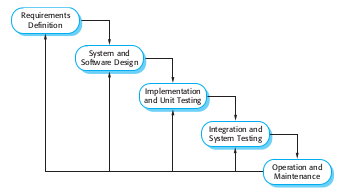
\includegraphics[scale=0.7]{img/wf.png}
        	\caption{Modello a cascata \label{fig:wf} }
        \end{figure}
        Vediamo una spiegazione più dettagliata:
        \begin{itemize}
        	\item \textbf{Requirements analysis and definition}: si stabiliscono servizi, limiti e fini del software consultandosi col cliente
        	\item \textbf{System and software design}: si stabilisce un'architettura di sistema complessiva stabilendo l'hardware e il software necessario
        	\item \textbf{Implementation and unit testing}: si sviluppano le unità di test e si verifica che ogni parte del software risponda alle specifiche richieste presa singolarmente
        	\item \textbf{Integration and system testing}: si testa il software nella sua interezza, si verifica che il software rispetti ogni requisito e infine si consegna il prodotto al cliente
        	\item \textbf{Operation and maintenance}: una volta che il prodotto è stato consegnato si provvede a mantenerlo, risolvendo eventuali errori e aggiungendo eventuali funzionalità, soddisfacendo eventuali nuovi requisiti. Potrebbe non essere uno step presente ogni volta
        \end{itemize}
    \item \textbf{modello iterativo (Iterative development)}: modello in cui le fasi di sviluppo avvengono
        nel corso del tempo, senza effettuare prima tutta la progettazione e poi l'implementazione, 
        sviluppando versioni sempre più definite del software, portando subito in risalta i problemi 
        e/o le mancate interpretazioni del sistema da sviluppare.\newline
        Prevede diverse implementazioni di questo modello, come ad esempio l'UP, lo Scrum e la modellazione
        agile, in cui il concetto di fondo è quello di conoscere, sviluppare e progettare il sistema a passi
        successivi, al fine di avere ad ogni passo un sottoinsieme del sistema già funzionante e questo
        permette di poter reagire ai cambiamenti dei requisiti e permettere una manutenzione
        mantenibile nel tempo.
    \item \textbf{ingegneria del Software basata sui componenti (CBSE)}
\end{enumerate}
\newpage
\subsubsection{Sviluppo incrementale}
Lo sviluppo incrementale si basa sull'idea di sviluppare un'implementazione iniziale del software che viene revisionata dai futuri utenti dello stesso. Si procede nella stessa maniera con ulteriori versioni fino a giungere ad un'implementazione finale. Quindi sviluppo, indicato in figura \figurename~\ref{fig:inc} e consegna sono strutturati in una sequenza di incrementi, ognuno delle quali corrisponde a parte delle funzionalità richieste, con ovviamente un ordine di priorità dato dal cliente (le prime parti conterranno le funzionalità principali del software).
\begin{figure}
	\centering
	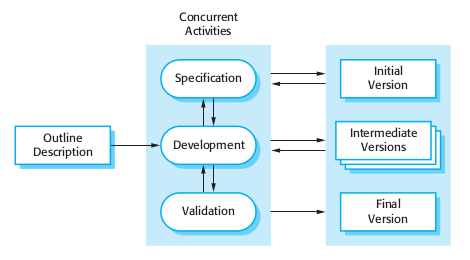
\includegraphics[scale=0.7]{img/inc.png}
	\caption{sviluppo incrementale \label{fig:inc} }
\end{figure}
Lo sviluppo incrementale ha 3 vantaggi principali rispetto 
al modello a cascata:
\begin{enumerate}
	\item si riduce il costo relativo al cambio di specifiche del cliente, riducendo anche la quantità di analisi e documentazione che andrebbe rielaborata
	\item si hanno feedback costanti sullo sviluppo grazie alla continua prova diretta delle varie implementazioni
	\item si può fornire gradualmente al cliente un software funzionante anche se privo di alcune features, di modo che possa usare parte del software ben prima del suo completo sviluppo
\end{enumerate}
Inoltre i rischi di fallimento si abbassano e i servizi a priorità più alta sono testati più a fondo. Del resto questo modello può essere rallentato facilmente da problemi burocratici. Inoltre il processo di sviluppo è più difficile da controllare da parte di un manager e il continuo aggiungere features può danneggiare l'architettura generale del software 
\textbf{pagina 34}










I metodi di ingegneria del software sono l'implementazione dei seguenti modelli generici, e nella
maggioranza si utilizza un modello iterativo, al fine di rendere incrementale lo sviluppo e ridurre
il rischio di fallimento del progetto.
\begin{center}
	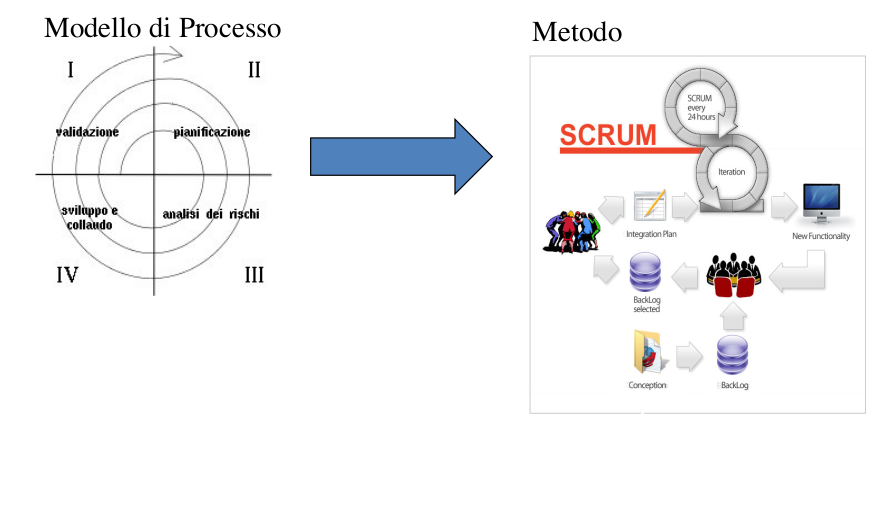
\includegraphics[scale=2.0]{img/ing.png}
\end{center}
% inizio sistemazione

si ha il seguente feedback del modello a cascata:
\begin{center}
\psscalebox{1.0 1.0} % Change this value to rescale the drawing.
{
\begin{pspicture}(0,-3.8)(15.6,3.8)
\psframe[linecolor=black, linewidth=0.04, dimen=outer](2.8,3.8)(0.0,2.6)
\psframe[linecolor=black, linewidth=0.04, dimen=outer](6.0,2.2)(2.8,1.0)
\psframe[linecolor=black, linewidth=0.04, dimen=outer](9.2,0.6)(6.0,-0.6)
\psframe[linecolor=black, linewidth=0.04, dimen=outer](12.4,-1.0)(9.2,-2.2)
\psframe[linecolor=black, linewidth=0.04, dimen=outer](15.6,-2.6)(12.4,-3.8)
\rput[bl](0.53333336,3.3){definizione}
\rput[bl](0.43333334,2.82){dei requisiti}
\rput[bl](2.8990476,1.76){progettazione}
\rput[bl](3.1866667,1.46){del sistema e}
\rput[bl](6.087619,0.0){implementazione}
\rput[bl](6.0804764,-0.44){e test delle unità}
\rput[bl](9.546667,-1.52){integrazione e }
\rput[bl](9.486667,-2.0){test del sistema}
\rput[bl](13.066667,-3.22){operatività}
\rput[bl](12.646667,-3.5){emanutenzione}
\rput[bl](3.58,1.14){del software}
\psline[linecolor=black, linewidth=0.04, arrowsize=0.05291667cm 2.0,arrowlength=1.4,arrowinset=0.0]{->}(12.4,-3.4)(1.2,-3.4)(1.2,2.6)
\psline[linecolor=black, linewidth=0.04, arrowsize=0.05291667cm 2.0,arrowlength=1.4,arrowinset=0.0]{->}(10.8,-3.4)(10.8,-2.2)
\psline[linecolor=black, linewidth=0.04, arrowsize=0.05291667cm 2.0,arrowlength=1.4,arrowinset=0.0]{->}(7.6,-3.4)(7.6,-0.6)
\psline[linecolor=black, linewidth=0.04, arrowsize=0.05291667cm 2.0,arrowlength=1.4,arrowinset=0.0]{->}(4.4,-3.4)(4.4,1.0)
\psline[linecolor=black, linewidth=0.04, arrowsize=0.05291667cm 2.0,arrowlength=1.4,arrowinset=0.0]{->}(2.8,3.4)(4.4,3.4)(4.4,2.2)
\psline[linecolor=black, linewidth=0.04, arrowsize=0.05291667cm 2.0,arrowlength=1.4,arrowinset=0.0]{->}(6.0,1.8)(7.6,1.8)(7.6,0.6)
\psline[linecolor=black, linewidth=0.04, arrowsize=0.05291667cm 2.0,arrowlength=1.4,arrowinset=0.0]{->}(9.2,0.2)(10.8,0.2)(10.8,-1.0)
\psline[linecolor=black, linewidth=0.04, arrowsize=0.05291667cm 2.0,arrowlength=1.4,arrowinset=0.0]{->}(12.4,-1.4)(14.0,-1.4)(14.0,-2.6)
\end{pspicture}
}
\end{center}
\begin{center}

	\psscalebox{1.0 1.0} % Change this value to rescale the drawing.
	{
		\begin{pspicture}(0,-2.55)(6.71,2.55)
			\rput[bl](0.0,2.25){requirements}
			\rput[bl](1.6,1.05){design}
			\rput[bl](2.4,-0.15){implementation}
			\rput[bl](4.0,-1.35){verification}
			\rput[bl](4.8,-2.55){maintenance}
			\psline[linecolor=black, linewidth=0.04, arrowsize=0.05291667cm 2.0,arrowlength=1.4,arrowinset=0.0]{->}(1.2,2.25)(2.0,1.45)
			\psline[linecolor=black, linewidth=0.04, arrowsize=0.05291667cm 2.0,arrowlength=1.4,arrowinset=0.0]{->}(2.4,1.05)(3.2,0.25)
			\psline[linecolor=black, linewidth=0.04, arrowsize=0.05291667cm 2.0,arrowlength=1.4,arrowinset=0.0]{->}(3.6,-0.15)(4.4,-0.95)
			\psline[linecolor=black, linewidth=0.04, arrowsize=0.05291667cm 2.0,arrowlength=1.4,arrowinset=0.0]{->}(4.8,-1.35)(5.6,-2.15)
		\end{pspicture}
	}

\end{center}
Invece di rilasciare il sistema in una singola consegna,
sviluppo e consegna sono strutturati in una sequenza di
incrementi, ognuno dei quali corrispondenti a parte
delle funzionalità richieste. Questa è la \textbf{consegna incrementale}. requisiti utente sono ordinati per priorità, i requisiti ad alta priorità sono inclusi nei primi incrementi.  \newpage
Una volta che lo sviluppo di un incremento inizia, i
requisiti sono congelati; invece possono evolvere i
requisiti per gli incrementi successivi:
\begin{center}
	\psscalebox{1.0 1.0} % Change this value to rescale the drawing.
	{
		\begin{pspicture}(0,-2.8)(16.05,2.8)
			\rput[bl](0.4,2.4){definizione}
			\rput[bl](0.4,2.0){sommaria}
			\rput[bl](0.4,1.6){dei requisiti}
			\rput[bl](4.4,2.4){assegnazione}
			\rput[bl](4.4,2.0){dei requisiti}
			\rput[bl](4.4,1.6){agli incrementi}
			\rput[bl](8.8,2.4){progettazione}
			\rput[bl](8.8,2.0){architettura}
			\rput[bl](8.8,1.6){di sistema}
			\rput[bl](0.4,-0.4){sviluppo}
			\rput[bl](0.4,-0.8){degli incrementi}
			\rput[bl](0.4,-1.2){di sistema}
			\rput[bl](4.8,-0.4){convalida}
			\rput[bl](4.8,-0.8){dell'incremento}
			\rput[bl](9.2,-0.4){integrazione}
			\rput[bl](9.2,-0.8){dell'incremento}
			\rput[bl](13.6,-0.4){validazione}
			\rput[bl](13.6,-0.8){del sistema}
			\rput[bl](14.0,1.6){sistema finale}
			\rput[bl](6.8,-2.8){sistema incompleto}
			\psframe[linecolor=black, linewidth=0.04, dimen=outer](2.8,2.8)(0.0,1.2)
			\psframe[linecolor=black, linewidth=0.04, dimen=outer](7.2,2.8)(4.0,1.2)
			\psframe[linecolor=black, linewidth=0.04, dimen=outer](11.2,2.8)(8.4,1.2)
			\psframe[linecolor=black, linewidth=0.04, dimen=outer](3.2,0.0)(0.0,-1.6)
			\psframe[linecolor=black, linewidth=0.04, dimen=outer](7.6,0.0)(4.4,-1.6)
			\psframe[linecolor=black, linewidth=0.04, dimen=outer](12.0,0.0)(8.8,-1.6)
			\psframe[linecolor=black, linewidth=0.04, dimen=outer](16.0,0.0)(13.2,-1.6)
			\psline[linecolor=black, linewidth=0.04, arrowsize=0.05291667cm 2.0,arrowlength=1.4,arrowinset=0.0]{->}(2.8,2.0)(4.0,2.0)
			\psline[linecolor=black, linewidth=0.04, arrowsize=0.05291667cm 2.0,arrowlength=1.4,arrowinset=0.0]{->}(7.2,2.0)(8.4,2.0)
			\psline[linecolor=black, linewidth=0.04, arrowsize=0.05291667cm 2.0,arrowlength=1.4,arrowinset=0.0]{->}(10.0,1.2)(10.0,0.8)(1.2,0.8)(1.2,0.0)
			\psline[linecolor=black, linewidth=0.04, arrowsize=0.05291667cm 2.0,arrowlength=1.4,arrowinset=0.0]{->}(3.2,-0.8)(4.4,-0.8)
			\psline[linecolor=black, linewidth=0.04, arrowsize=0.05291667cm 2.0,arrowlength=1.4,arrowinset=0.0]{->}(7.6,-0.8)(8.8,-0.8)
			\psline[linecolor=black, linewidth=0.04, arrowsize=0.05291667cm 2.0,arrowlength=1.4,arrowinset=0.0]{->}(12.0,-0.8)(13.2,-0.8)
			\psline[linecolor=black, linewidth=0.04, arrowsize=0.05291667cm 2.0,arrowlength=1.4,arrowinset=0.0]{->}(14.8,-1.6)(14.8,-2.4)(2.0,-2.4)(2.0,-1.6)
			\psline[linecolor=black, linewidth=0.04, arrowsize=0.05291667cm 2.0,arrowlength=1.4,arrowinset=0.0]{->}(14.8,0.0)(14.8,1.6)
		\end{pspicture}
	}

\end{center}
Con la consegna incrementale si hanno i seguenti vantaggi:
\begin{itemize}
	\item funzioni utili per il cliente possono essere rilasciate ad ogni incremento, quindi alcune funzionalità di sistema sono disponibili sin dai primi incrementi
	\item i primi incrementi rappresentano dei prototipi che supportano la scoperta dei requisiti per i successivi incrementi
	\item i rischi di fallimento si abbassano
	\item i servizi a priorità più alta tendono ad essere collaudati più a fondo
\end{itemize}
Se si ha che i requisiti vengono scoperti attraverso lo sviluppo si ha lo \textbf{sviluppo evoluzionistico}. Si usano prototipi che poi non verranno utilizzati nel corso del progetto vero e proprio\\
\begin{center}
	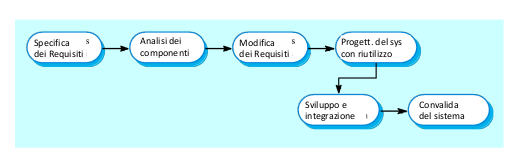
\includegraphics[scale=0.7]{img/ms.png}
\end{center}
Si ha ingegneria del software basata su componenti se si hanno già librerie su cui lavorare.\\
Passiamo al primo modello iterativo, quello di B. Boehm.
\begin{center}
	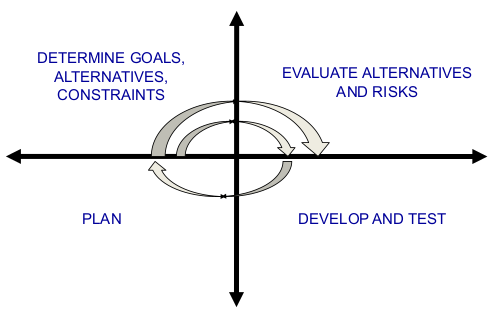
\includegraphics[scale=0.7]{img/ms2.png}
\end{center}
si parte dal quadrante in alto a sinistra e si arriva al prodotto finale mediante una serie di iterazioni. Si sceglie ovviamente la soluzione più sicura. I vari passaggi sono qui rappresentati:
\begin{center}
	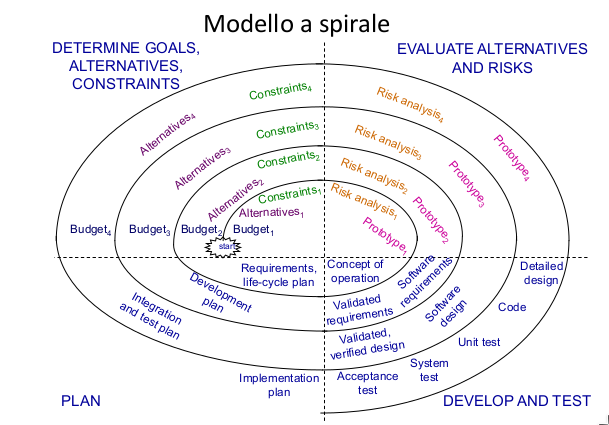
\includegraphics[scale=0.7]{img/ms3.png}
\end{center}
\section{Modello UP}
Il metodo di modellazione UP(Unified Process), conosciuto anche come RUP(Rational Unified Process), è un
processo iterativo molto diffuso per lo sviluppo software, in cui sono presenti degli elementi tratti da 
altri metodi, come Extreme Programming, Scrum e così via.

Lo sviluppo iterativo
Si hanno i modelli agili, che si basano sulla \textbf{consegna incrementale}. Si hanno iterazioni brevi e timeboxed, con un raffinamento evolutivo di piani, dei requisiti e del progetto. Questi metodi favoriscono la collaborazione nei gruppi e la riduzione dei costi.
\subsection{Modello UP o RUP}
Il metodo UP, \textit{inified process}, conosciuto anche come RUP, \textit{Rational Unified Process}, usa la notazione UML, \textit{unified modeling language} ed è uno dei più importanti modelli agili. È è un processo iterativo e incrementale. Si basa sulla suddivisone di un grande processo in iterazioni controllate. Si hanno passi piccoli, timeboxed da 2 a 6 settimane, feedback rapito e adattamento, di requisiti, modelli, stime di sviluppo e costi e priorità.
\begin{center}
	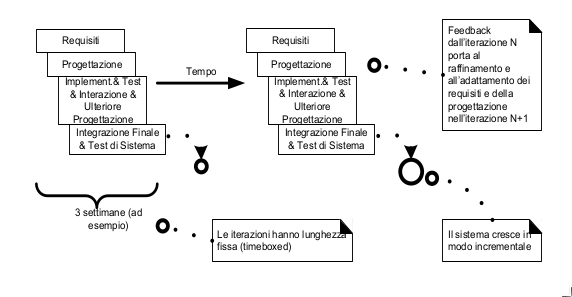
\includegraphics[scale=0.7]{img/ms4.png}
\end{center}
Si hanno 4 fasi nel modello RUP:
\begin{enumerate}
	\item \textbf{avviamento:} dove viene stabilita la “bussines rationale” del progetto e stabiliti gli obiettivi, stime dei costi e dei tempi. Si ha uno studio di fattibilità, \textit{Life-Cycle Objective Milestone}
	\item \textbf{elaborazione}: dove si raccolgono i requisiti in modo più dettagliato, si procede con l'analisi ad alto livello per stabilire l'architettura di base e vengono analizzati i rischi principali. Si hanno stime più affidabili: \textit{Life-Cycle Architecture Milestone}
	\item \textbf{costruzione} che consiste di molte iterazioni, e ad ogni iterazione viene costruita una parte del sistema che soddisfa un sottoinsieme di requisiti. Viene effettuato il testing e l'integrazione. Si ha la preparazione al rilascio: \textit{Initial Operational Capability Milestone}
	\item \textbf{transizione:} dove vengono affrontati tutti gli aspetti legati al fine-tuning delle funzionalità,
	      prestazioni, qualità, beta-testing, ottimizzazione, formazione degli
	      utenti,... È la \textit{Product Release Milestone}
\end{enumerate}
\begin{center}
	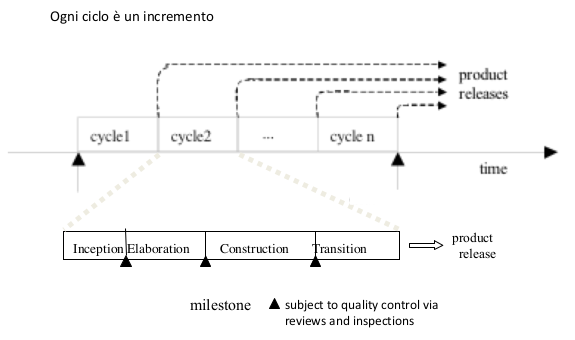
\includegraphics[scale=0.7]{img/ms5.png}
\end{center}
Si hanno i seguenti vantaggi dello sviluppo iterativo:
\begin{itemize}
	\item minore chance di fallimento del progetto
	\item riduzione precoce dei rischi
	\item progresso visibile
	\item feedback precoce e coinvolgimento dell'utente
	\item "abbracciare il cambiamento"
\end{itemize}
\begin{center}
	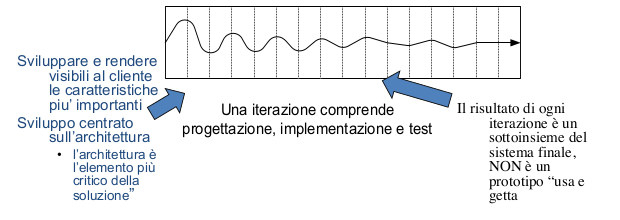
\includegraphics[scale=0.7]{img/ms6.png}
\end{center}
Vediamo un esempio con 5 iterazioni:
\begin{center}
	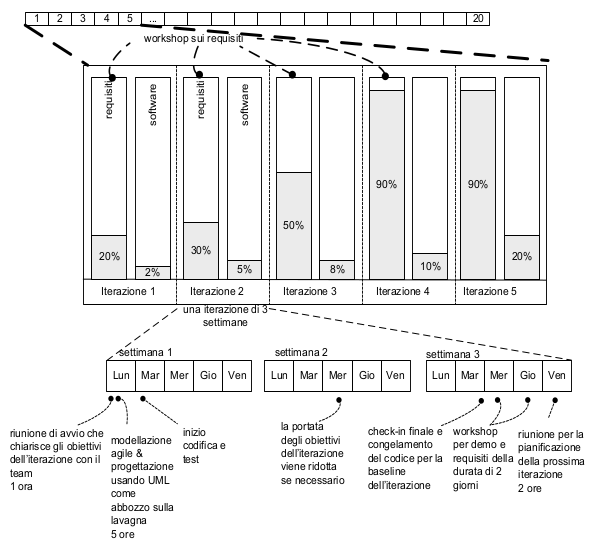
\includegraphics[scale=0.7]{img/ms7.png}
\end{center}
\newpage
vediamo un'altra rappresentazione del ciclo di sviluppo:
\begin{center}
	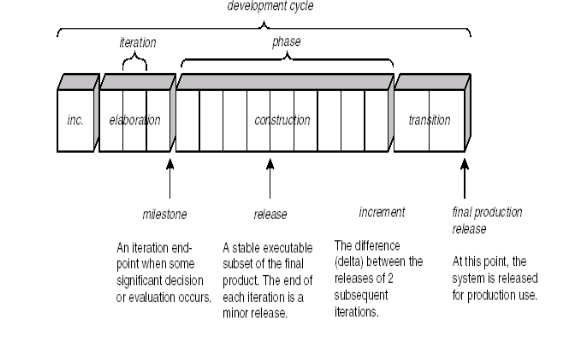
\includegraphics[scale=0.65]{img/ms8.png}
\end{center}
vediamo anche un'immagine per rappresentare l'organizzazione del processo, con fasi, iterazioni e "discipline":
\begin{center}
	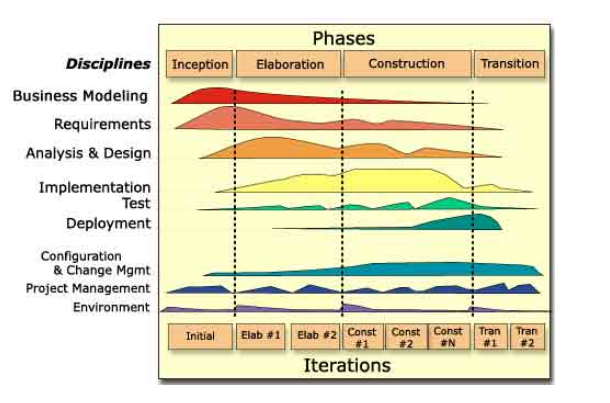
\includegraphics[scale=0.65]{img/ms9.png}
\end{center}
tra le discipline troviamo analisi e progettazione
%approfondire su libro
Si hanno le seguenti caratteristiche principlai per l?UP:
\begin{itemize}
	\item è iterativo e incrementale
	\item si enfasi sul modello invece che sul linguaggio naturale
	\item è centrato sull'architettura
\end{itemize}
\subsection{Processo Scrum}
Iniziamo con un'immagine che rappresenta questo metodo agile:
\begin{center}
	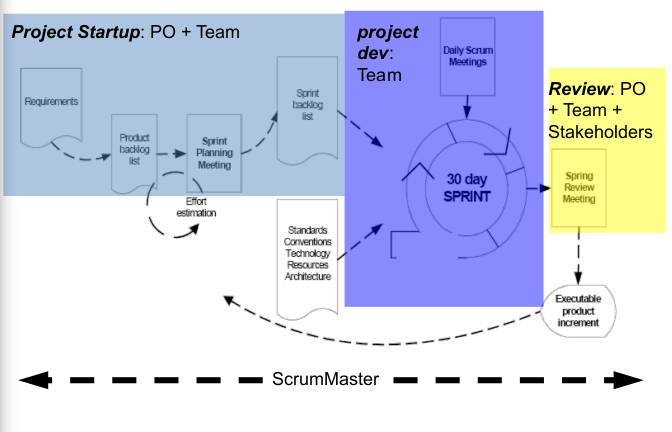
\includegraphics[scale=0.65]{img/ms10.png}
\end{center}
È un processo iterativo basato sull controllo dello stato di
avanzamento. Si hanno i seguenti principi fondamentali:
\begin{itemize}
	\item \textbf{visibilità:} gli aspetti significativi del processo di sviluppo devono essere visibili a tutti e tutti gli aspetti devono essere chiari
	\item \textbf{ispezione:} poter ispezionare frequentemente il lavoro fatto per verificare che si sta procedendo verso gli
	      obiettivi posti
	\item \textbf{adattamento}, se si sta deviando dagli obiettivi, occorre un adattamento per minimizzare altre deviazioni. Deve essere svolto nel minor tempo possibile in caso di necessità
\end{itemize}
Si hanno i seguenti ruoli:
\begin{itemize}
	\item \textbf{product owner} che si occupa della definizione delle
	      caratteristiche del progetto da sviluppare (1 sola
	      persona, e.g. committente, o altri...); gestisce il
	      Product Backlog. Lavora costantemente col team
	\item \textbf{team:} dedicato allo sviluppo e rilascio del
	      prodotto attraverso incrementi successivi (da 3 a
	      7/8 membri)
	\item \textbf{scrum master:} responsabile che lo SCRUM venga
	      applicato correttamente. Non è un project manager, fa da intermezzo tra team e product owner, collabora col team etc
\end{itemize}
Ecco un'immagine che rappresenta lo sviluppo con Scrum:
\begin{center}
	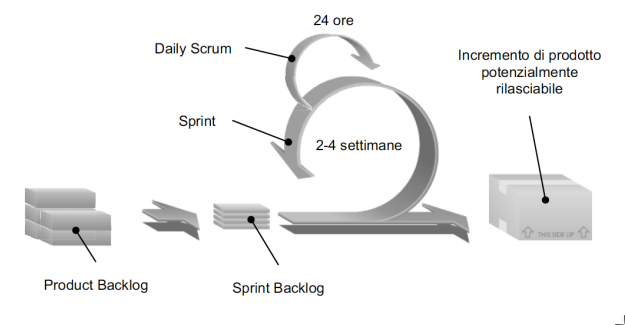
\includegraphics[scale=0.7]{img/ms11.png}
\end{center}
SI hanno quindi:
\begin{itemize}
	\item releases brevi con sottoinsiemi consegnati velocemente
	\item in ogni istante si hanno test eseguibili, non si ha logica duplicata e si ha un numero minimo di features
	\item si ha \textit{refactoring }con miglioramento continuo
	\item si un testo continuo e automatico, \textit{testing first}
	\item si hanno due sviluppatori che lavorano insieme, \textit{pair programming}
	\item il codice è proprietà del team e non del singolo dev, \textit{collective owbership}
	\item si hanno check-in frequenti e integrazioni continue, \textit{continuous integration}
	\item il cliente lavora col team
\end{itemize}
I \textbf{requisiti} sono una descrizione dei servizi del sistema e dei suoi vincoli operativi. Si hanno due tipi di requisiti:
\begin{itemize}
	\item \textbf{requisiti utenti:} affermazioni in linguaggio naturale, corredate da tabelle e diagrammi, riguardanti i servizi che il sistema offre ed i vincoli operazionali. Sono scritti per i clienti e sono da loro comprensibili anche se non	hanno conoscenze tecniche dettagliate.\\

	\item \textbf{requisiti di sistema:} un documento strutturato che definisce in modo dettagliato le funzioni del sistema, i servizi ed i vincoli operazionali. Definisce cosa deve essere implementato, quindi può essere parte del
	      contratto tra acquirente e sviluppatore. È la base del progetto della soluzione e può essere illustrato utilizzando i \textbf{modelli di sistema}.

\end{itemize}
i requisiti possono avere 3 problemi:
\begin{itemize}
	\item \textbf{ambiguità:} il sistema fornisce visualizzazioni appropriate per leggere i documenti
	\item \textbf{incompletezza:} i requisiti devono descrivere tutti i	servizi forniti dal sistema (anche se in realtà tutto ciò è impossibile, per questo esistono i cambiamenti)
	\item \textbf{inconsistenza}: le descrizioni non devono contenere conflitti o contraddizioni (anche questa cosa è difficilissima da ottenere)
\end{itemize}
SI hanno anche i \textbf{requisiti funzionali} servizi che il sistema deve (o non deve) fornire. Si hanno anche i \textit{requisiti non funzionali}, come vincoli sui servizi temporali, standard, sull'usabilità etc... I requisiti non funzionali possono essere più critici dei requisiti funzionali: \textbf{se non sono soddisfatti il sistema è spesso inutilizzabile}. Si hanno alcuni requisiti non funzionali:
\begin{itemize}
	\item \textbf{prodotto: }specificano che il prodotto deve comportarsi in un modo particolare
	      esempi: velocità di esecuzione, affidabilità.\\
	      \textit{L’interfaccia utente sarà implementata con HTML semplice senza frames
		      e applets}
	\item \textbf{organizzativi: }conseguenza di politiche e procedure dell’organizzazione del cliente e dello sviluppatore.
	      esempi: linguaggio di programmazione, metodo di sviluppo.\\
	      \textit{Il processo di sviluppo e la relativa documentazione sarà conforme alle
		      norme XYZCo-SP-STAN-95}
	\item \textbf{esterni: }provengono da fattori esterni al sistema e al processo di sviluppo.
	      esempi: interoperabilità, leggi e norme.
	      \\ \textit{Il sistema non deve rilevare agli operatori nessuna informazione
		      personale sui clienti oltre al nome e al numero di riferimento}
\end{itemize}
\begin{center}
	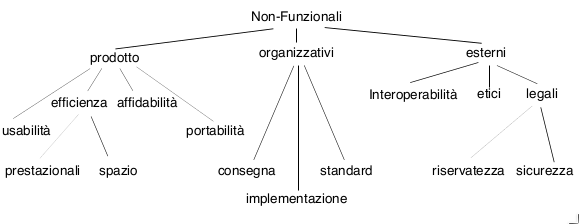
\includegraphics[scale=0.8]{img/req.png}
\end{center}
\newpage
Tutto ciò perché il linguaggio naturale presenta mancanza di chiarezza, ambiguità, confusione etc... Esistono alternative:
\begin{center}
	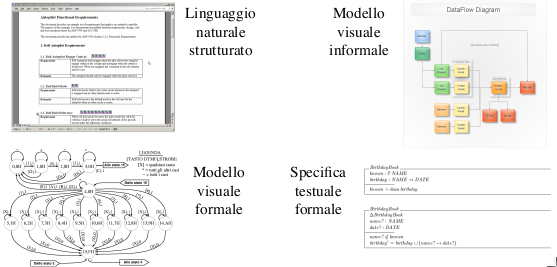
\includegraphics[scale=0.8]{img/req2.png}
\end{center}
I requisiti hanno un formato standard, usano il linguaggio in modo consistente, evitano il gergo tecnico e evidenziano delle porzioni di testo per identificare le parti più importanti dei requisiti. Un esempio di standard è quello IEEE830.\\
I casi d'uso possono essere visualizzati con l'UML:
\begin{center}
	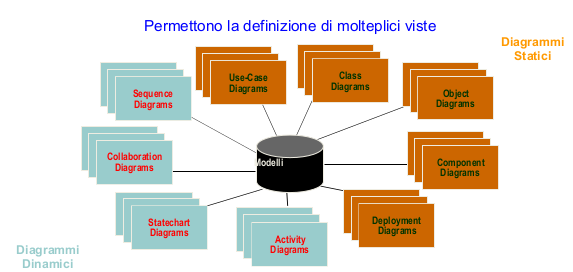
\includegraphics[scale=0.8]{img/uml.png}
\end{center}

\chapter{Casi d'uso}
\begin{center}
	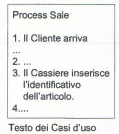
\includegraphics[scale=0.7]{img/casdi.png}
\end{center}
\textit{I casi d'uso sono storie scritte, testuali, di qualche attore che usa un sistema per raggiungere degli obbiettivi}. I casi d'uso possono a loro volta influenzare molti altri elaborati dell'analisi, progettazione, implementazione, gestione del progetto e test. Passiamo a qualche definizione:
\begin{itemize}
	\item un \textbf{attore} è qualcosa 6 qualcuno dotato di
		comportamento, come una persona (caratterizzata da un ruolo), un sistema informatico o un'organizzazione
	\item uno \textbf{scenario o istanza di caso d'uso} è una sequenza specifica di azioni e interazioni
		  tra il sistema e alcuni attori. Uno scenario descrive una particolare storia nell'uso del sistema, o un percorso attraverso il caso d'uso
\end{itemize}
\textit{Informalmente }un caso d'uso quindi può essere definito come una collezione di scenari correlati, di successo e fallimento, che descrivono un attore che usa un sistema per raggiungere un obiettivo.\\
\textbf{UP} definisce il modello di caso nell'ambito della disciplina dei Requisiti. Inoltre \textbf{i casi d'uso sono documenti di testo, non diagrammi, e la modellazione dei casi
d'uso è innanzitutto un atto di scrittura di testi, non di disegno di diagrammi}. Il Modello dei Casi d'Uso può includere, opzionalmente, un diagramma UML dei casi
d'uso che mostra i nomi dei casi d'uso e degli attori, nonché le relazioni tra di essi. Esso costituisce un buon diagramma di contesto di un sistema e del suo ambiente, oltre a
costituire un indice di facile consultazione dei nomi dei casi d'uso. Si ricorda che \textbf{i casi d'uso non sono orientati ad oggetti}.\\
I casi d'uso sono un buon metodo per mantenere la semplicità e consentire agli esperti
di dominio o ai fornitori di requisiti di scrivere essi stessi i casi d'uso, o perlomeno partecipare alla loro scrittura. Un altro valore dei casi d'uso è che mettono in risalto gli obiettivi e il punto di vista
dell'utente.\\
I casi d'uso sono requisiti, soprattutto requisiti funzionali o comportamentali, che indicano che cosa farà il sistema. In UP e in molti metodi moderni, i casi d'uso sono il meccanismo
centrale che viene consigliato per la scoperta e la definizione dei requisiti.\\
Torniamo a parlare di attori. Un attore è qualcosa o qualcuno dotato di comportamento, Anche il sistema in discussione,\textit{ SuD, da system under discussion}, stesso è un attore, quando ricorre ai servizi di altri sistemi. Si hanno tre tipi di attori correlati al SuD:
\begin{enumerate}
	\item \textbf{attore primario} che raggiunge degli obiettivi utente utilizzando i servizi del SuD. Identificare gli attori primari è utile per trovare gli obiettivi degli utenti,che guidano i casi d'uso
	\item \textbf{attore di supporto} che offre un servizio (per esempio, informazioni) al SuD. Spesso è un sistema informatico, ma potrebbe essere un'organizzazione o una
	persona. Identificare gli attori di supporto è utile per chiarire le interfacce esterne e i loro protocolli
	\item \textbf{attore fuori scena} che ha un interesse nel comportamento del caso d'uso, ma non è
	un attore primario o di supporto. Identificare gli attori fuori scena è utile per garantire che tutti gli interessi necessari vengano individuati e soddisfatti. Gli interessi degli attori fuori scena sono spesso sottili o facili da tralasciare, a meno che gli attori stessi non vengano esplicitamente nominati
\end{enumerate}
Si hanno inoltre tre diversi livelli di \textbf{formalità} per i casi d'uso:
\begin{enumerate}
	\item \textbf{formato breve} ovvero un riepilogo conciso di un solo paragrafo, normalmente relativo al
	solo scenario principale di successo. Si usa durante l'analisi iniziale dei requisiti, per capire rapidamente l'argomento e la portata. È possibile scriverlo in pochi minuti
	\item \textbf{formato informale} ovvero più paragrafi, scritti in modo informale, relativi a vari scenari. Si usa come il formato breve ma qui si ha un livello di dettaglio maggiore
	\item \textbf{formato dettagliato} dove tutti i passi e le variazioni sono scritti nel dettaglio; ci sono anche delle sezioni di supporto, come le pre-condizioni e le garanzie di successo. Va usato opo che molti casi d'uso sono stati identificati e scritti in formato breve, alcuni casi d'uso (circa il 10\%) che hanno maggior valore e che sono più significativi dal punto di vista dell'architettura vengono scritti in formato dettagliato. Si ha quindi:
	\begin{center}
		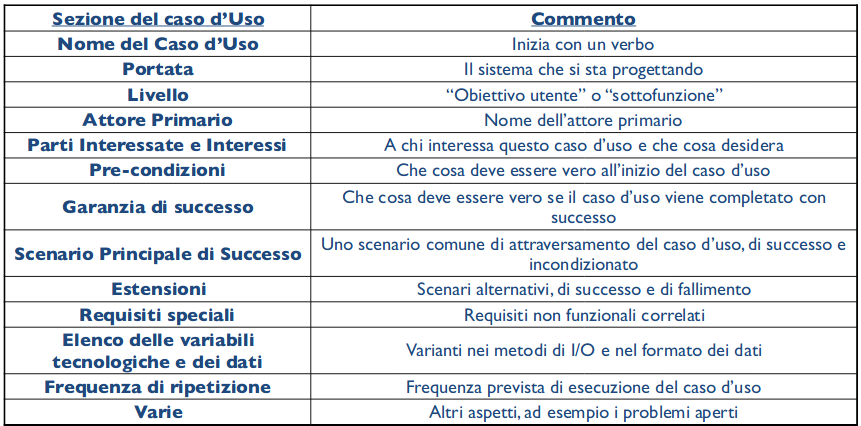
\includegraphics[scale=0.5]{img/det.png}
	\end{center}
\end{enumerate}
Parliamo ora di scenari. Si hanno due tipologie:
\begin{enumerate}
	\item \textbf{scenario principale (di successo)} che descrive un percorso di successo tipico che soddisfa gli interessi delle parti interessate. Si noti che spesso non comprende alcuna condizione o diramazione. Questo rende il caso d'uso più comprensibile e più estensibile. È formato da una sequenza di passi:
	\begin{enumerate}
		\item un'interazione tra attori
		\item una validazione (solitamente effettuata dal sistema
		\item un cambiamento di stato da parte del sistema
	\end{enumerate}
	Il primo passo di un caso d'uso non rientra sempre in questa classificazione, ma può indicare l'evento (trigger) che scatena l'esecuzione dello scenario. I nomi degli attori vengono di solito scritti con l'iniziale maiuscola, per facilitarne l'identificazione. Un esempio:
	\begin{center}
		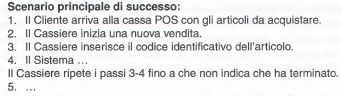
\includegraphics[scale=1.1]{img/pri.png}
	\end{center}
	\item \textbf{scenari alternativi (o flussi alternativi o estensioni)} che descrivono tutte le diramazioni e gli altri scenari, sia di successo che di fallimento. La loro stesura è spesso lunga e complessa. Nella scrittura completa dei casi d'uso, la combinazione del flusso di base e degli altri scenari descritti dalle estensioni dovrebbe soddisfare "quasi" tutti gli interessi delle parti interessate. Tuttavia, alcuni interessi possono essere descritti come requisiti non funzionali, e pertanto riportati nelle Specifiche Supplementari piuttosto che nei casi d'uso. Gli scenari relativi alle estensioni sono diramazioni dello scenario principale di successo, e vengono indicati con riferimento ai suoi passi. Si contrassegnano con una lettera posta dopo il numero che identifica il passo (per il passo 3 si avrà 3a, 3b etc...) inoltra prima riporta la condizione, poi la reazione. Per esempio:
	\begin{center}
		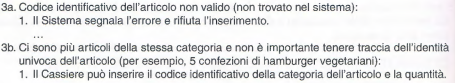
\includegraphics[scale=0.9]{img/alt.png}
	\end{center}
	Un estensione è costituita da condizione e gestione. La gestione di un'estensione può essere riassunta in un unico passo, oppure può comprendere una sequenza di passi. Al termine della gestione di un'estensione, per default lo scenario si fonde di nuovo con lo scenario principale di successo, a meno che l'estensione non indichi diversamente (per esempio, l'arresto del sistema). In alcuni casi, i punti di estensione sono abbastanza complessi. Questo può essere un motivo per esprimere l'estensione come un caso d'uso separato.
\end{enumerate}
Un caso d'uso può diramarsi in un altro caso d'uso e in effetti, i casi d'uso vengono spesso scritti come ipertesti, e l'esecuzione di un altro caso d'uso viene rappresentata come un collegamento ipertestuale. In questo caso, facendo clic sul nome del caso d 'uso sottolineato, ne verrà visualizzato il testo.\\
Se un requisito non funzionale, un attributo di qualità o un vincolo si riferiscono in modo specifico a un caso d' uso, allora è bene registrarlo insieme al caso d'uso. Potrebbe trattarsi di qualità come prestazioni, affidabilità e usabilità, oppure di vincoli di progettazione, che siano stati imposti o considerati probabili. Si hanno quindi i \textbf{requisiti speciali}.
\newpage
Vediamo ora un esempio completo di caso d'uso:
\begin{center}
	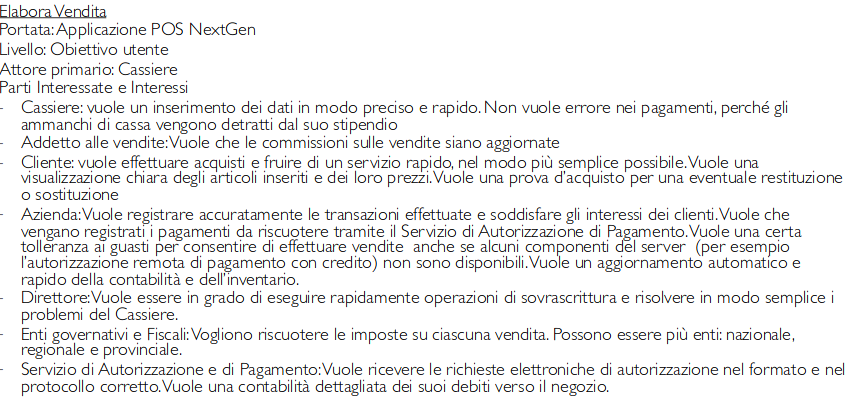
\includegraphics[scale=0.57]{img/ca1.png}
\end{center}
\begin{center}
	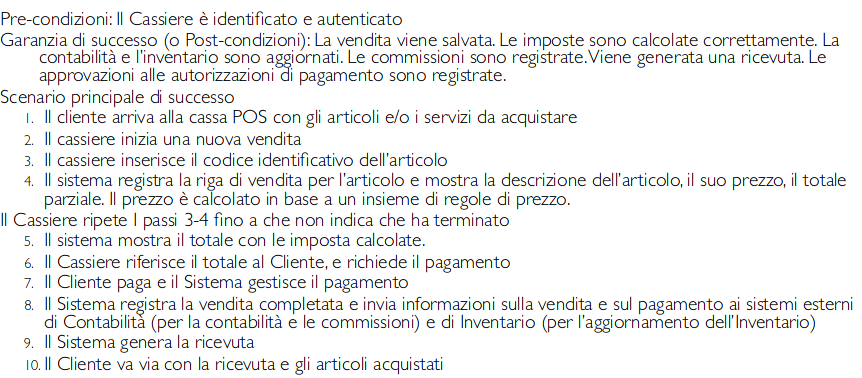
\includegraphics[scale=0.57]{img/ca2.png}
\end{center}
\begin{center}
	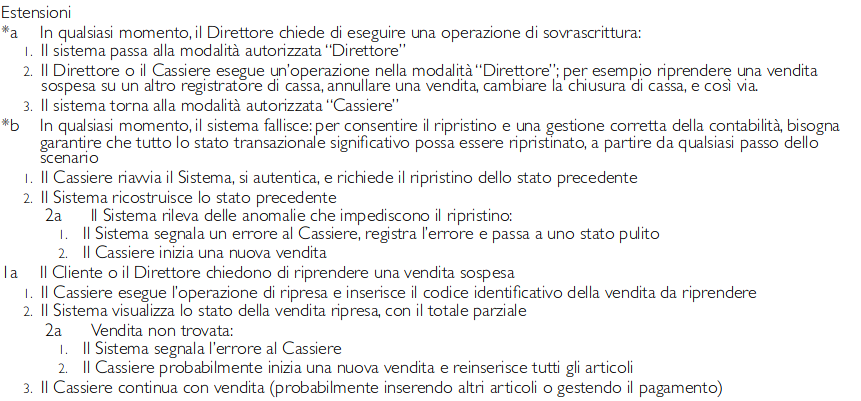
\includegraphics[scale=0.57]{img/ca3.png}
\end{center}
\begin{center}
	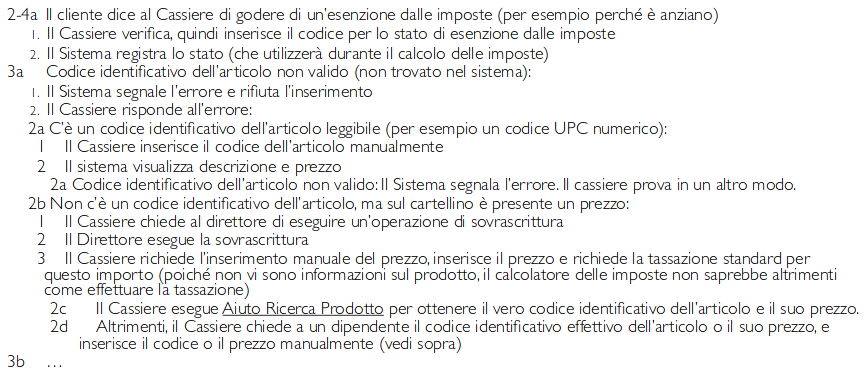
\includegraphics[scale=0.57]{img/ca4.png}
\end{center}
\begin{center}
	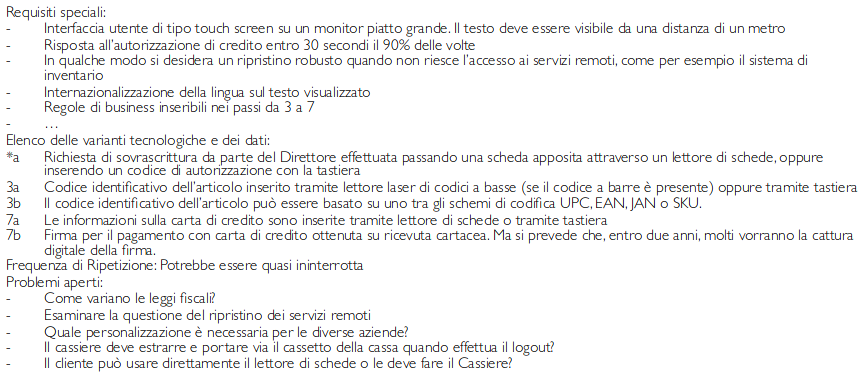
\includegraphics[scale=0.57]{img/ca5.png}
\end{center}
Si hanno delle linee guida per la stesura dei casi d'uso. Si cerca uno stile essenziale, ignorando l'interfaccia utente e concentrandosi sullo scopo dell'attore, ignorando come un sistema fa qualcosa ma concentrandosi su cosa deve fare. Per facilitare la lettura dei requisiti, è perciò opportuno scrivere i casi d'uso in modo conciso, e allo stesso tempo in modo completo (con una chiara indicazione di soggetto  verbo e di eventuali frasi subordinate).\\
I \textbf{casi d'uso a scatola nera }sono il tipo più comune e consigliato; non descrivono il funzionamento interno del sistema, i suoi componenti o aspetti relativi al suo progetto. Piuttosto, il sistema è descritto come dotato di responsabilità. Questa è una metafora comune e unificante nel pensare orientato agli oggetti; gli elementi software hanno responsabilità e collaborano con altri elementi dotati di responsabilità. Usando i casi d'uso a scatola nera per definire le responsabilità del sistema, è possibile specificare che cosa deve fare il sistema (comportamento o requisiti funzionali) senza decidere come lo farà (progettazione). In effetti, la definizione dell'"analisi" rispetto alla "progettazione" è talvolta riassunta come "che cosa" rispetto a "come". Questo è un tema importante nello sviluppo del software: durante l'analisi dei requisiti bisogna specificare il comportamento esterno del sistema, considerato a scatola nera, evitando di prendere decisioni sul "come". Successivamente, durante la progettazione, andrà creata una soluzione che soddisfa le specifiche. 
\newpage
Per esempio:
\begin{center}
	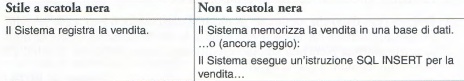
\includegraphics[scale=0.7]{img/box.png}
\end{center}
È anche importante trovare i casi d'uso e si ha una procedura di base per farlo:
\begin{enumerate}
	\item scegliere i confini del sistema, ovvero definire il sistema al meglio. Per chiarire la definizione dei confini del sistema in corso di progettazione, è utile sapere che gli attori primari e gli attori di supporto sono considerati esterni al sistema. Una volta identificati gli attori esterni, i confini diventano più chiari.
	\item identificare gli attori primari. Alcune volte sono gli obiettivi a svelare gli attori, o viceversa. Si possono usare una serie di domande per facilitare l'operazione:
	\begin{center}
		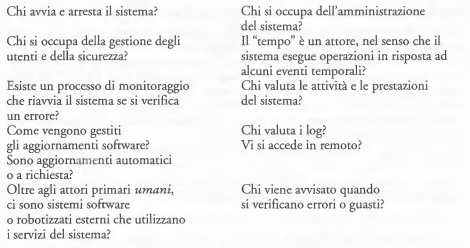
\includegraphics[scale=0.7]{img/dom.png}
	\end{center}
	\item identificare gli obiettivi di ciascun attore primario. Si crea quinid un elenco attori-obiettivi, tipo questo:
	\begin{center}
		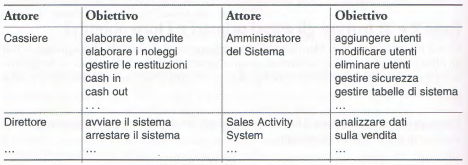
\includegraphics[scale=0.7]{img/atob.png}
	\end{center}
	inoltre risulta più producente, nella realtà, chiedere all'attore stesso quale sia il suo obbiettivo. \\
	Un altro approccio per trovare attori, obiettivi e casi d'uso è basato sull'identificazione di eventi esterni. Spesso un gruppo di eventi appartiene allo stesso caso d'uso. Per esempio:
	\begin{center}
	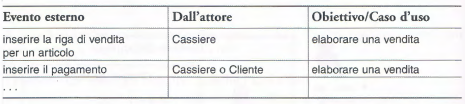
\includegraphics[scale=0.7]{img/atob2.png}
	\end{center}
	\item definire i casi d'uso che soddisfano gli obiettivi degli utenti; il loro nome va scelto in base all'obiettivo. Di solito, i casi d'uso a livello di obiettivo utente saranno in corrispondenza biunivoca con gli obiettivi degli utenti. 
\textbf{Il nome dei casi d'uso deve iniziare con un verbo e, in generale va definito un caso d'uso per ciascun obiettivo utente.} È opportuno assegnare al caso d'uso un nome simile all'obiettivo dell'utente. \\ \textit{un'eccezione comune alla scelta di un caso d'uso per obiettivo è quella che riunisce gli obiettivi separati CRUD (acronimo di create, retrieve, update, delete, ovvero creare, leggere, aggiornare, eliminare) in un unico caso d'uso CRUD, chiamato Gestisci <X>. Per esempio, gli obiettivi "modifica utente" , "elimina utente" e così via sono tutti soddisfatti dal caso d'uso Gestisci Utenti.}
\end{enumerate}
\textbf{Naturalmente, nello sviluppo iterativo ed evolutivo, non tutti gli obiettivi o i casi d'uso
saranno identificati completamente o correttamente fin dall'inizio. Anche la scoperta dei
requisiti è evolutiva}.\\
Bisogna poi verificare la validità dei casi d'uso. Si hanno quindi tre test:
\begin{itemize}
	\item \textbf{test del capo}: \textit{il capo vi chiede: "Cosa avete fatto tutto il giorno?" e voi rispondete: "Il login!". Il vostro capo sarà felice?}. Se non lo è il caso d'uso non supera il test del capo, il che significa che non è fortemente mirato a ottenere risultati il cui valore sia misurabile. Potrebbe essere un caso d'uso a un livello più basso, ma non al livello a cui è desiderabile concentrarsi durante l'analisi dei requisiti. Ciò non significa che bisogna sempre ignorare i casi d'uso che non superano il test del capo
	\item \textbf{test EBP (\textit{Elementary Business Process})}, che deriva dall'ingegneria dei processi di business: \textit{Un processo di business elementare è un'attività svolta da una persona in un determinato tempo e luogo, in risposta a un evento di business, che aggiunge un valore di business misurabile e lascia i dati in uno stato coerente; per esempio, "Approva un credito" o "Stabilisci il prezzo per un ordine"}. Come nella definizione di UP, enfatizza l'aggiunta di un valore di business osservabile o misurabile, e giunge a una situazione in cui il sistema e i dati sono in uno stato stabile e coerente. \textbf{Il test EBP è simile al test del capo, soprattutto in termini di qualifica in termini di valore aziendale misurabile.}
	\item \textbf{test della dimensione}, che si basa sul fatto che un caso d'uso è formato da diversi passi (e nel complesso si hanno da 3 a 10 pagine di testo). Un errore comune nella modellazione dei casi d'uso è definire un caso d'uso a sé formato da un singolo passo.
\end{itemize}
\textbf{Ci potrebbero essere delle eccezioni a questi test.}
\section{Diagrammi dei casi d'uso}
UML fornisce una notazione dei diagrammi dei casi d'uso che consente di illustrare i nomi e gli attori dei casi d'uso, nonché le relazioni tra gli stessi, per esempio:
\begin{center}
	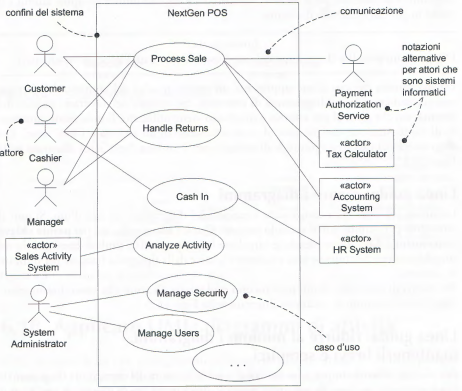
\includegraphics[scale=0.7]{img/casd.png}
\end{center}
\newpage
\textbf{I diagrammi dei casi d'uso e le relazioni tra casi d'uso sono secondari nel lavoro che
riguarda i casi d'uso. I casi d'uso sono documenti di testo. Lavorare sui casi d'uso significa scrivere testo.} \\
Un diagramma dei casi d'uso rappresenta un ottimo quadro del contesto del sistema; esso costituisce un buon diagramma di contesto, che consiste nel mostrare i confini del sistema, ciò che giace al suo esterno e come esso viene utilizzato. È utile come strumento di comunicazione che riassume il comportamento di un sistema e i suoi attori.\\
\textit{Per ribadire, il lavoro importante dei casi d'uso è la scrittura del testo, non i diagrammi o le relazioni tra casi d'uso. Se un'organizzazione spreca molte ore (o peggio ancora, giorni) a lavorare su un diagramma dei casi d' uso e a discutere le relazioni tra casi d'uso anziché concentrarsi sulla scrittura del testo, vuol dire che il tempo è stato impiegato male}.\\
A livello di notazione si ha:
\begin{itemize}
	\item \textbf{gli attori} sono rappresentati da un omino, col nome scritto sotto:
	\begin{center}
		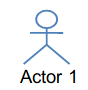
\includegraphics[scale=0.7]{img/act.png}
	\end{center}
	\item \textbf{i casi d'uso} sono rappresentati con un ovale contenente la dicitura del caso d'uso:
	\begin{center}
		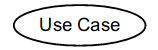
\includegraphics[scale=0.7]{img/dcas.png}
	\end{center}
	\newpage
	\item \textbf{le associazioni} sono canali di comunicazione tra attore e caso d'uso. Si hanno due rappresentazioni:
	\begin{enumerate}
		\item \textbf{una linea continua direzionata}, per specificare chi da inizio all'interazione
		\item \textbf{una linea continua non direzionata}, per indicare che entrambe le parti possono dare inizio ad un'interazione
	\end{enumerate}
	\begin{center}
		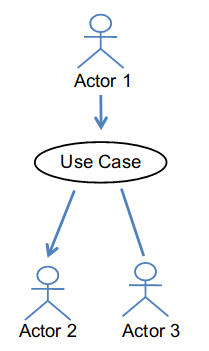
\includegraphics[scale=0.7]{img/asso.png}
	\end{center}
	\item \textbf{l'include (inclusione)} si rappresenta con una linea tratteggiata direzionata con l'indicazione \textit{<<include>>} e indica la relazione tra un caso d'uso base ed un caso d'uso incluso nel caso d'uso base:
	\begin{center}
		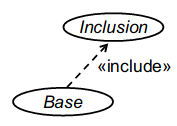
\includegraphics[scale=0.7]{img/incd.png}
	\end{center}
	\begin{center}
		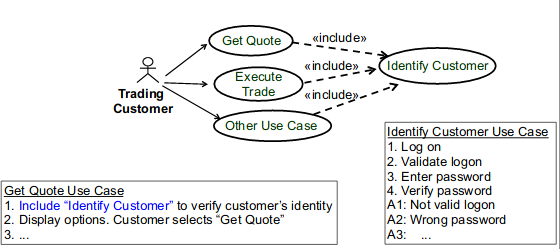
\includegraphics[scale=0.7]{img/incd2.png}
	\end{center}
	\textit{il caso d'uso è eseguito completamente quando viene raggiunto il punto di inclusione}
	\item \textbf{l'extend (estensione)}, si rappresenta come l'include (specificando \textit{<<extend>>}) e connette un caso d'uso esteso ad un caso d'uso base. Aggiunge varianti ad un caso d’uso base e viene inserito solo se la condizione di estensione è vera. Si hanno estensioni inserite solo in corrispondenza degli extension point:
	\begin{center}
		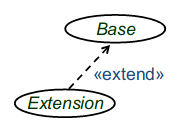
\includegraphics[scale=0.7]{img/extd.png}
	\end{center}
	\begin{center}
		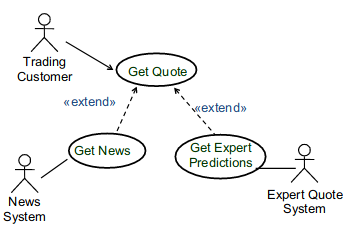
\includegraphics[scale=0.7]{img/extd2.png}
	\end{center}
	\begin{center}
		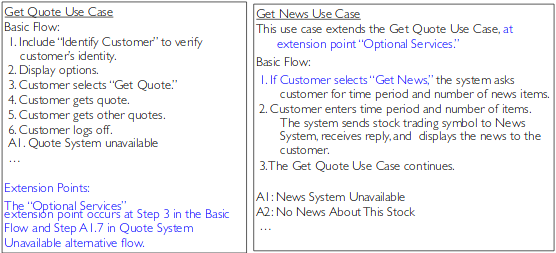
\includegraphics[scale=0.7]{img/extd3.png}
	\end{center}
	\textit{Il caso d'uso esteso è eseguito quando il punto di estensione è raggiunto e la condizione di estensione è vera}
	\item \textbf{la generalization (generalizzazione)} si ha quando un caso d'uso base è una generalizzazione di un caso d'uso child. Viene rappresentata con una linea continua direzionata con la freccia non riempita:
	\begin{center}
		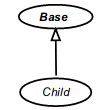
\includegraphics[scale=0.7]{img/gend.png}
	\end{center}
	\textit{Il caso d'uso generalizzato viene eseguito se la condizione di generalizzazione è vera} inoltre \textit{la generalizzazione è puramente concettuale, non ci sono regole da seguire, come ad esempio l'utilizzo di punti di estensione}. Si ha:
	\begin{center}
		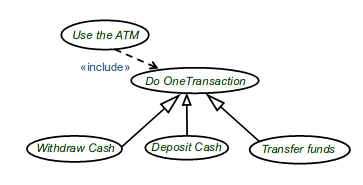
\includegraphics[scale=0.7]{img/gend2.png}
	\end{center}\begin{center}
		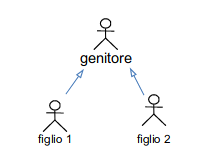
\includegraphics[scale=0.7]{img/gend3.png}
	\end{center}\begin{center}
		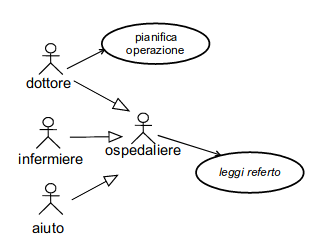
\includegraphics[scale=0.7]{img/gend4.png}
	\end{center}
	
\end{itemize}
\begin{shaded}
Anche se gli elenchi dettagliati di funzioni non sono consigliabili, le funzionalità del
sistema possono essere riassunte in modo utile in un \textit{elenco di caratteristiche} chiaro, ad
alto livello, chiamato caratteristiche di sistema, come parte del documento di Visione. Contrariamente alle caratteristiche di basso livello, costituite da molte pagine, un elenco di caratteristiche di sistema dovrebbe comprende solo alcune decine di voci. Esso fornisce un riepilogo conciso delle funzionalità del sistema, indipendente dalla vista dei casi d'uso, come nel seguente esempio. Talvolta i casi d'uso non sono adatti; alcune applicazioni richiedono un punto di vista guidato dalle caratteristiche. Per esempio, i server applicativi, i sistemi di gestione di basi di dati e altri sistemi di middleware o di back-end vanno piuttosto descritti e si evolvono in termini di caratteristiche ("supporto per i Web Services nella prossima versione"). I casi d'uso non sono idonei a queste applicazioni o al modo in cui esse~evolvono in termini di forze del mercato.
\end{shaded}
\newpage
I casi d'uso sono fondamentali in UP e in molti altri metodi iterativi. UP incoraggia lo sviluppo guidato dai casi d'uso. Si ha quindi:
\begin{itemize}
	\item i requisiti funzionali sono registrati principalmente nei casi d'uso (Modello dei Casi d'Uso); le altre tecniche per i requisiti (come l'elenco delle funzioni) sono secondarie, o addirittura non utilizzate
	\item i casi d'uso rivestono un ruolo importante nella pianificazione iterativa. Il lavoro di un'iterazione è definito, in parte, scegliendo alcuni scenari di casi d'uso o interi casi d'uso. I casi d'uso sono inoltre un input fondamentale per stimare costi e tempi di un progetto
	\item la progettazione è guidata da realizzazioni di casi d'uso; il team progetta oggetti e sottosistemi che collaborano che consentono di eseguire o realizzare i casi d'uso
	\item i casi d'uso spesso influenzano l'organizzazione dei manuali per l'utente
	\item i test funzionali o di sistema corrispondono agli scenari dei casi d'uso
	\item è possibile creare nella UI "creazioni guidate" (wizard) o scelte rapide (shortcut) per facilitare le attività comuni degli scenari dei casi d'uso più comuni e importanti
\end{itemize}
\chapter{Contratti delle Operazioni}
\begin{center}
	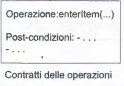
\includegraphics[scale=0.7]{img/opid.png}
\end{center}
In UP, i \textbf{casi d'uso} e le \textbf{caratteristiche di sistema} sono i modi principali per descrivere il comportamento del sistema. Normalmente sono sufficienti, ma talvolta è utile una descrizione più dettagliata o precisa del comportamento del sistema. I contratti delle operazioni usano pre-condizione e post-condizione per descrivere nel dettaglio i cambiamenti agli oggetti in un modello di dominio, come risultato di un'operazione di sistema.\\
I contratti delle operazioni possono essere considerati parte del Modello dei Casi d'Uso, poiché forniscono maggiori dettagli dell'analisi sull'effetto delle operazioni di sistema implicate dai casi d'uso.\\
Definiamo le sezioni di un contratto:
\begin{itemize}
	\item \textbf{operazione:} nome e parametri dell'operazione
	\item \textbf{riferimenti:} casi d'uso in cui può verificarsi questa operazione
	\item \textbf{pre-condizioni: }ipotesi significative sullo stato del sistema o degli oggetti nel Modello di Dominio prima dell'esecuzione dell'operazione. Sono ipotesi non banali.
	\item \textbf{post-condizioni: }è la sezione più importante ovvero lo stato degli oggetti nel Modello di Dominio dopo il completamento dell'operazione. Le post-condizioni descrivono i cambiamenti nello stato degli oggetti nel modello di dominio. I cambiamenti di stato nel modello di dominio comprendono le istanze create, le associazioni formate o rotte e gli attributi modificati. Le post-condizioni non sono azioni da eseguire nel corso dell'operazione; si tratta piuttosto di osservazioni (rilevazioni) sugli oggetti del modello di dominio che risultano avere al termine dell'operazione. Si dividono in:
	\begin{itemize}
		\item creazione o cancellazione di un'istanza
		\item cambiamento del valore di un attributo
		\item associazioni (collegamenti in UML) formate o spezzate
	\end{itemize}
	\textbf{Le post-condizioni non sono sempre necessarie}. \textit{Le post-condizioni vanno espresse con un verbo al passato, per sottolineare che si tratta di osservazioni dei cambiamenti di stato provocati da un'operazione, e non di un'azione che deve accadere}
\end{itemize}
I contratti delle operazioni possono essere definiti per le \textbf{operazioni di sistema}, ovvero operazioni che il sistema, considerato come un componente a scatola nera, offre nella sua interfaccia pubblica. Le operazioni di sistema possono essere identificate mentre si abbozzano gli SSD, \textit{diagrammi di sequenza di sistema}.
\newpage
Un evento di sistema di input implica che il sistema contenga un'operazione di sistema per gestire quell'evento,
così come un messaggio OO (che è un tipo di evento o segnale) viene gestito da un metodo OO (che è un tipo di operazione):
\begin{center}
	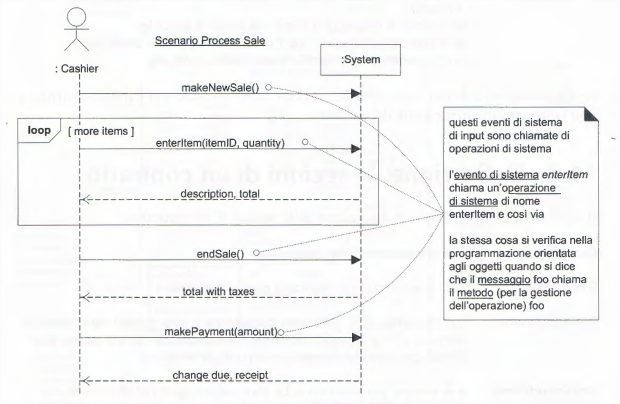
\includegraphics[scale=0.7]{img/oo.png}
\end{center}
L'intero insieme delle operazioni di sistema, tra tutti i casi d'uso, definisce l'interfaccia
di sistema pubblica, considerando il sistema come un singolo componente o una singola classe. In UML, il sistema nel suo insieme può essere rappresentato come un unico oggetto di una classe denominata, per esempio, System.\\
Durante la creazione dei contratti è normale che emerga la necessità di registrare nuove classi concettuali, attributi o associazioni nel modello di dominio. Non ci si limiti alla formulazione fatta in precedenza del modello di dominio; la si deve ampliare man mano che si fanno nuove scoperte.Nei metodi iterativi ed evolutivi (che riflettono la realtà dei progetti software), tutti gli elaborati dell'analisi e della progettazione sono considerati parziali e imperfetti, ed evolvono in risposta a nuove scoperte.\\
In UP, i casi d'uso sono il repository principale dei requisiti del progetto. Essi possono fornire tutti i dettagli, o la maggior parte di essi, necessari per sapere che cosa fare durante la progettazione; in questo caso i contratti non sono d'aiuto. Tuttavia ci sono situazioni in cui non è opportuno descrivere nei casi d' uso tutti i dettagli e la complessità dei cambiamenti di stato richiesti, poiché risulterebbero troppo dettagliati.
\\
Si ha la seguente linea guida per creare contratti:
\begin{itemize}
	\item identificare le operazioni di sistema dagli SSD
	\item creare un contratto per le operazioni di sistema complesse o i cui effetti sono probabilmente sottili, o che non sono chiare dai casi d'uso
	\item descrivere le post-condizioni con le seguenti categorie:
	\begin{itemize}
		\item creazione o cancellazione di istanza
		\item modifica di attributo
		\item associazione formata o spezzata
	\end{itemize}
\end{itemize}
\textit{Il problema più comune è dimenticarsi di includere la formazione di associazioni. In particolare quando sono creare nuove istanze, è molto probabile che debbano essere stabilire delle associazioni con diversi oggetti.}\\
\section{Operazioni e UML}
UML definisce formalmente la nozione di \textbf{operazione}: \textit{un'operazione è una specifica di una trasformazione o di una interrogazione che un oggetto può essere chiamato ad eseguire.}\\
In UML sono operazioni, per esempio, gli elementi di un'interfaccia. Sono quindi \textbf{astrazioni} e non implementazioni. In UML, invece, un \textbf{metodo} è:
\textit{l'implementazione di un'operazione. Esso specifica l'algoritmo o la procedura associata a un'operazione}.\\
Nel metamodello di UML, un'operazione ha una \textbf{firma} (o signature, con nome e parametri) e, cosa più importante in questo contesto, è associata a un insieme di oggetti UML di tipo Constraint (Vincolo) classificati come pre-condizioni e post-condizioni che specificano la semantica dell'operazione.
UML definisce la semantica delle operazioni attraverso i vincoli, che possono essere specificati nello stile delle pre-condizioni e post-condizioni. Si noti che, come sottolineato in questo capitolo, la specifica di un'operazione UML non può mostrare un algoritmo o una soluzione, ma solo i cambiamenti di stato o gli effetti dell'operazione. Oltre a utilizzare i contratti per specificare le operazioni pubbliche dell'intero sistema (ovvero, le operazioni di sistema), i contratti possono essere applicati alle operazioni a qualsiasi livello di granularità: le operazioni pubbliche (o l'interfaccia) di un sottosistema, di un componente, di una classe astratta, e così via. Per esempio, è possibile definire operazioni per una singola classe software, per esempio Stack. Le operazioni a grana grossa discusse in questo capitolo appartengono a una classe System che rappresenta l'intero sistema considerato come componente a scatola nera, ma in UML le operazioni possono appartenere a qualsiasi classe o interfaccia, tutte con le relative pre-condizioni e post-condizioni.
\chapter{Modellazione di Dominio}
Un \textbf{modello di dominio} è il modello più importante e classico dell'analisi OO; esso illustra i concetti significativi di un dominio. Può fungere da sorgente di ispirazione perla progettazione di alcuni oggetti software.\\
\textbf{Come tutte le cose nella modellazione agile e nello spirito di UP, il modello di dominio è opzionale.}
Il modello di dominio a sua volta può influenzare i contratti delle operazioni, il glossario e il Modello di Progetto, in particolare gli oggetti software nello strato del dominio del Modello di Progetto.\\
Vediamo un piccolo esempio:
\begin{center}
	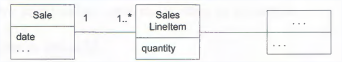
\includegraphics[scale=0.7]{img/domd.png}
\end{center}
L'immagine mostra un modello di dominio parziale, disegnato con la notazione di un diagramma delle classi di UML. L'applicazione della notazione dei diagrammi delle classi di UML per un modello di dominio produce un modello secondo un punto di vista concettuale:
\begin{center}
	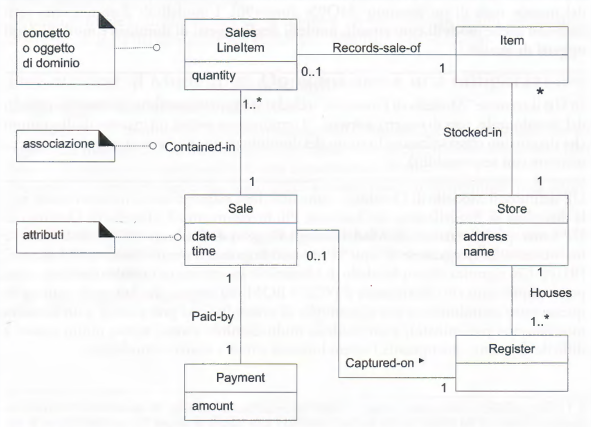
\includegraphics[scale=0.6]{img/domd2.png}
\end{center}
Quindi un \textbf{modello di dominio} è \textit{una rappresentazione visuale di classi concettuali o di oggetti del mondo reale di un dominio}. \textit{In UP, il termine "Modello di Dominio" indica una rappresentazione di classi concettuali del mondo reale, non di oggetti software. Il termine "non" indica un insieme di diagrammi che descrivono classi software, lo strato del dominio di un'architettura software o oggetti software con responsabilità.} Si ha che il Modello di Dominio di UP è una specializzazione del \textit{Modello degli Oggetti di Business}.\\
Applicando la notazione UML, un modello di dominio è illustrato con un insieme di diagrammi delle classi in cui non sono definite operazioni (firme di metodi). Esso fornisce un punto di vista concettuale e può mostrare:
\begin{itemize}
	\item oggetti di dominio o classi concettuali
	\item associazioni tra classi concettuali
	\item attributi di classi concettuali
\end{itemize}
Ovviamente quanto espresso con la notazione UML poteva essere espresso come testo semplice nel Glossario di UP. Un Modello di Dominio UP è una visualizzazione di oggetti del mondo reale in un dominio di interesse, \textbf{non} di oggetti software.\\
Si indica quindi con \textbf{strato di dominio} il secondo significato di modello di dominio, orientato agli oggetti software, come avviene comunemente.\\
Il modello di dominio illustra \textbf{classi concettuali}. Una \textbf{classe concettuale}, informalmente, è un'idea, una cosa, o un oggetto, formalmente, può essere considerata in termini del suo simbolo, della sua intensione e della sua estensione: 
\begin{itemize}
	\item \textbf{simbolo:} parole o immagini che rappresentano una classe concettuale
	\item \textbf{intensione:} la definizione di una classe concettuale
	\item \textbf{estensione:} l'insieme di esempi a cui la classe concettuale si applica
\end{itemize}
Ovvero:
\begin{center}
	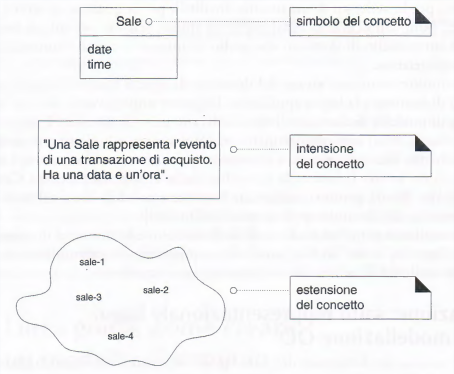
\includegraphics[scale=0.7]{img/conc.png}
\end{center}
\textbf{Un modello di dominio non è un modello di dati}. Non si deve dunque escludere una classe semplicemente perché i requisiti non indicano alcuna necessità ovvia di ricordare informazioni sulla stessa (un criterio comune nella modellazione dei dati perla progettazione di basi di dati relazionali, ma irrilevante nella modellazione di dominio)oppure perché la classe concettuale non ha attributi.\\
Vediamo le linee guida per creare un modello di dominio. Si hanno i seguenti passo:
\begin{enumerate}
	\item trovare le classi concettuali. Si hanno tre strategie utili per trovarle:
	\begin{enumerate}
	\item riusare o modificare dei modelli esistenti. Questo è il primo approccio, il migliore e generalmente il più facile dal quale iniziare, se possibile
	\item utilizzare un elenco di categorie:
	\begin{center}
		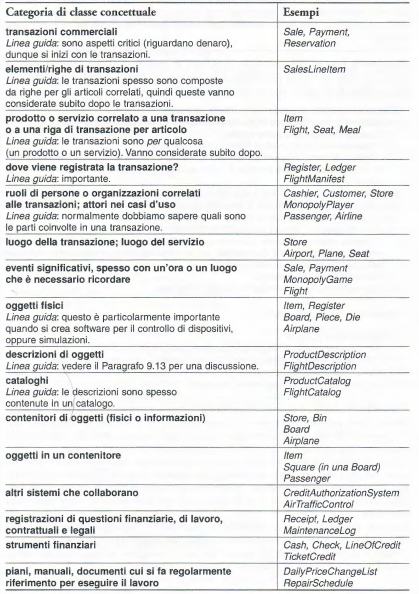
\includegraphics[scale=0.7]{img/catd.png}
	\end{center}
	\item identificare nomi e locuzioni nominali. Si usa quindi l'\textbf{analisi linguistica}. È basata sull'identificazione di nomi e di locuzioni nominali (ovvero, di frasi oggetti formate da un nome principale insieme ai suoi aggettivi e determinanti) nelle descrizioni testuali di un dominio; questi vengono poi considerati come classi concettuali candidate o attributi. \textbf{Occorre prestare particolare attenzione con questo metodo; una corrispondenza meccanica da nome a classe non è possibile, poiché le parole nel linguaggio naturale sono
ambigue.}
\end{enumerate}	 
	\item disegnarle come classi in un diagramma delle classi UML
	\item aggiungere associazioni e attributi
\end{enumerate}
\textit{Il modello di dominio è una visualizzazione di concetti e terminologia di dominio significativi.}
\\
Uno degli errori più comuni durante la creazione di un modello di dominio è quello di rappresentare qualcosa come un attributo mentre dovrebbe essere rappresentato come
una classe concettuale. Si ha quindi una regola per evitare questo: \textit{se nel mondo reale non pensiamo a una determinata classe concettuale X come a un numero o a un testo, allora probabilmente X è una classe concettuale, non un attributo}.\\
Analizziamo ora le \textbf{classi descrizione}. Una classe descrizione contiene informazioni che descrivono qualcos'altro. Può infatti accadere che ci sia necessità che alcuni oggetti siano descrizioni (talvolta chiamate
specifiche) di qual cos'altro. La necessità di classi descrizione è comune nei domini relativi a vendite, prodotti e servizi. È comune anche nella produzione, che richiede una descrizione di un prodotto manufatto, che è distinta dal prodotto stesso. Aggiungere una classe descrizione è necessario nei seguenti casi:
\begin{itemize}
	\item quando è necessaria una descrizione di un articolo o servizio, indipendentemente dall'attuale esistenza di istanze di tali articoli o servizi
	\item quando l'eliminazione delle istanze degli oggetti che descrivono darebbe luogo a una perdita di informazioni che invece è necessario conservare, ma che sono state erroneamente associate all'oggetto eliminato
	\item quando si vogliono ridurre le informazioni ridondanti o ripetute
\end{itemize}
\newpage
vediamo un esempio:
\begin{center}
	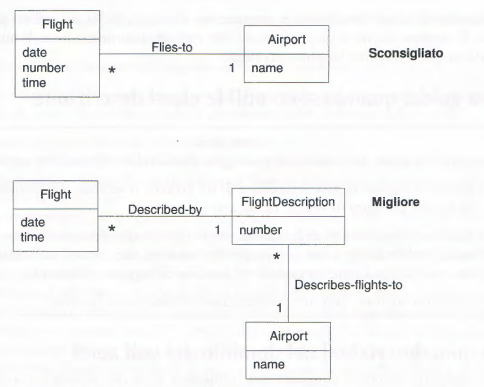
\includegraphics[scale=0.7]{img/carad.png}
\end{center}
\section{Associazioni}
\textbf{Un'associazione} è una relazione tra classi (più precisamente, tra istanze di queste classi)
che indica una connessione significativa e interessante.\\
In UML è definita come \textit{la relazione semantica tra due o più classificatori che comporta connessioni tra le rispettive istanze}.\\
Le associazioni che è utile mostrare sono solitamente quelle che implicano la conoscenza di una relazione che deve essere memorizzata per una certa durata di tempo, che a seconda del contesto potrebbe essere di millisecondi o di anni.\\ Si hanno due tipi di associazioni da includere nel modello di dominio:
\begin{enumerate}
	\item associazioni per cui la conoscenza della relazione deve essere conservata per una qualche durata
	\item associazioni derivate dall'elenco di associazioni comuni
\end{enumerate}
\textbf{È bene evitare di inserire troppe associazioni in un modello di dominio.} Si ricorda che in un grafo con $n$ nodi ci possono essere $\frac{n(n-1)}{2}$ associazioni tra nodi distinti, questo implica che si può rischiare di incappare in problematiche di "disturbo visivo", che diminuisce la leggibilità del diagramma stesso.\\
\subsection{Notazione per le Associazioni}
Un'associazione è rappresentata da una linea che collega le classi partecipanti; il nome di un'associazione ha l'iniziale maiuscola, per differenziarle dalle classi, che hanno l'iniziale maiuscola. La estremità di un'associazione possono contenere un'espressione di molteplicità, che indica le relazioni numeriche tra le istanze delle classi.
Un'associazione è per natura bidirezionale, nel senso che è possibile una navigazione logica dalle istanze di una delle due classi a quelle dell'altra, e viceversa. Questa navigazione è puramente astratta, \textbf{non è un'affermazione su connessioni tra entità software}.
\begin{center}
	\includegraphics[scale=0.7]{img/asd1.png}
\end{center}
Una "freccia della direzione di lettura" opzionale indica la direzione di lettura del nome dell'associazione; non indica una direzione di visibilità o di navigabilità. Se la freccia non è presente, la convenzione è di leggere l'associazione da sinistra verso destra oppure dall'alto verso il basso, anche se ciò non costituisce una regola in UML.\\
Normalmente si assegna il nome a un'associazione in base al formato \textit{NomeClasse-LocuzioneVerbale-NomeClasse}, in cui la locuzione verbale (ovvero, una frase formata da un verbo principale, più eventuali complemento, oggetto e avverbi) crea una sequenza leggibile e significativa.
\newpage
Ciascuna estremità di un'associazione è detta ruolo e può avere, opzionalmente:
\begin{itemize}
	\item espressione di molteplicità. La molteplicità definisce quante istanze di una classe A possono essere associate a un'istanza di una classe B, in un particolare momento, piuttosto che in un arco di tempo:
	\begin{center}
		\includegraphics[scale=0.7]{img/muld.png}
	\end{center}
	Si hanno diversi valori per una molteplicità:
	\begin{center}
		\includegraphics[scale=0.7]{img/muld2.png}
	\end{center}
	\item nome
	\item navigabilità
\end{itemize}
Si possono avere due classi collegate da più associazioni:
\begin{center}
		\includegraphics[scale=0.7]{img/muld3.png}
\end{center}
\subsection{Aggregazione e composizione}
L'\textbf{aggregazione} è un tipo di associazione che suggerisce la relazione \textit{intero-parte}. Se ne sconsiglia l'uso ma presenta la seguente notazione:
\begin{center}
	\includegraphics[scale=2.7]{img/aggd.png}
\end{center}
La \textbf{composizione}, nota anche come \textit{aggregazione composta}, è un forte tipo di aggregazione di tipo \textit{intero-parte} e implica che:
\begin{itemize}
	\item ciascuna istanza della parte appartiene ad una sola istanza del composto alla volta
	\item ciascuna parte appartiene sempre ad un composto
\end{itemize}
Si ha la seguente notazione:
\begin{center}
	\includegraphics[scale=0.7]{img/compd.png}
\end{center}
\section{Attributi}
Un \textbf{attributo} è un valore logico (un dato) di un oggetto. Vanno inclusi gli attributi he i requisiti (per esempio, i casi d' uso) suggeriscono o di cui
implicano una necessità di ricordare informazioni.\\
In UML gli attributi sono mostrati nella seconda sezione del rettangolo per una classe, opzionalmente è possibile anche mostrare il loro tipo e altre informazioni:
\begin{center}
	\includegraphics[scale=0.7]{img/attd.png}
\end{center}
Si ha però una sintassi completa:
\begin{center}
	\textit{visibility name : type multiplicity = default { property-string }}
\end{center}
per esempio:
\begin{center}
	\includegraphics[scale=0.7]{img/attd2.png}
\end{center}
Convenzionalmente, la maggior parte dei modellatori assume che gli attributi hanno una visibilità privata(indicata col "-"), a meno che sia mostrato diversamente, e pertanto normalmente non viene disegnato un simbolo esplicito per la visibilità. Tra le stringhe di proprietà per gli attributi, la più comune è probabilmente {readOnly},
che indica un attributo di sola lettura (una costante). È possibile usare una molteplicità per indicare la presenza opzionale per un valore, o il numero di oggetti che possono appartenere a un attributo collezione.\\
\begin{shaded}
Alcuni modellatori accettano che queste specifiche siano
lasciate solo nel modello di dominio; questo però è un metodo dispersivo e che può por-
tare a errori, poiché ci sono persone che tendono a non guardare il modello di dominio
in modo dettagliato o come guida per i requisiti (e magari non mantengono nemmeno
un modello di dominio).
Al contrario, si suggerisce di riportare tutti questi requisiti relativi agli attributi nel Glossario di UP, usato come dizionario dei dati. Magari è stata impiegata un'ora ad abbozzare
un modello di dominio con un esperto del dominio; dopodiché è utile impiegare ancora
15 minuti per esaminarlo e trasferire nel Glossario i requisiti implicati per gli attributi.
Un'altra alternativa è quella di utilizzare uno strumento che integri i modelli UML con
un dizionario dei dati; quindi tutti gli attributi appariranno automaticamente come voci
del dizionario.
\end{shaded}
Si possono avere attributi derivati:
\begin{center}
	\includegraphics[scale=0.7]{img/attd3.png}
\end{center}
In modo informale, la maggior parte degli attributi dovrebbe essere di un tipo di dato considerato "primitivo", come per esempio numeri e booleani. Normalmente, il tipo di
un attributo non dovrebbe essere un concetto complesso del dominio complesso, classi concettuali vanno correlate con associazioni non con attributi:
\begin{center}
	\includegraphics[scale=0.7]{img/attd4.png}
\end{center}
\begin{center}
	\includegraphics[scale=0.7]{img/attd5.png}
\end{center}
nello specifico un \textbf{tipo di dato} è rappresentato da tipi "primitivi" quali numeri,
booleani, caratteri, stringhe ed enumerazioni (come Size = {small, large}). Più precisamente, questo termine in UML indica un insieme di valori la cui identità univoca non
è significativa (nel contesto del nostro modello o sistema). In altre parole, i test di uguaglianza non sono basati sull'identità, bensì sul valore. \textbf{In altre parole, i test di uguaglianza non sono basati sull'identità, bensì sul valore.}\\
È possibile definire nuovi tipi di dato:
\begin{center}
	\includegraphics[scale=0.7]{img/datd.png}
\end{center}
\newpage
e si ha la seguente rappresentazione:
\begin{center}
	\includegraphics[scale=0.7]{img/datd2.png}
\end{center}
li attributi non dovrebbero essere usati per correlare classi concettuali nel modello
di dominio. La violazione più comune di questo principio consiste nell'aggiungere un
attributo chiave esterna, come viene fatto normalmente nella progettazione delle basi
di dati relazionali per correlare due tipi:
\begin{center}
	\includegraphics[scale=0.7]{img/datd3.png}
\end{center}
La maggior parte delle quantità numeriche non dovrebbe essere rappresentata come dei semplici numeri. Solitamente è buona pratica associare le unità di misura.\\
Nel complesso un modello di dominio risulterà:
\begin{center}
	\includegraphics[scale=0.7]{img/complex.png}
\end{center}
\begin{shaded}
Anche se paradossalmente sono state dedicate molte pagine alla spiegazione della mo-
dellazione di dominio, nelle mani degli esperti lo sviluppo di un modello (parziale,
evolutivo) in ciascuna iterazione può durare anche solo 30 minuti, o ancora meno se si
utilizzano dei pattern di analisi predefiniti.
Nello sviluppo iterativo, si fa evolvere un modello di dominio in modo incrementale su
diverse iterazioni. In ciascuna di esse, il modello di dominio è limitato agli scenari pre-
cedenti e corrente presi in considerazione, anziché estendersi a un modello "big bang"
di tipo a cascata che tenti di catturare dall'inizio tutte le possibili classi concettuali e
relazioni.
\end{shaded}
\chapter{Progettazione a Oggetti}
Esistono 3 modi per progettare ad oggetti:
\begin{enumerate}
	\item \textbf{codifica}, ovvero progettare mentre si codifica (in Java, C\#, ... ), possibilmente insieme a strumenti potenti come il refactoring. Dal modello mentale al codice.
	\item \textbf{disegno e poi codifica}, ovvero disegnare alcuni diagrammi UML su una lavagna o con uno strumento CASE per UML, poi passare alla codifica usando un IDE "testuale"
	\item \textbf{solo disegno}, 
\end{enumerate}
Alcuni degli scopi della modellazione agile sono ridurre il costo aggiuntivo del disegno e modellare per comprendere e comunicare, anziché per documentare. Le pratiche comprendono l'utilizzo di molte lavagne bianche (dieci in una stanza, non due) o di speciali fogli di plastica bianca
aderenti tramite carica statica (che hanno la stessa funzione di una lavagna) per ricoprire ampie aree delle pareti, l'utilizzo di pennarelli, fotocamere digitali e stampanti per catturare "UML come abbozzo", uno dei tre modi per applicare UML. Si ha inoltre la modellazione insieme agli altri e il creare diversi modelli in parallelo (lavorando per tot tempo ad un diagramma su una lavagna e poi un altro po' su un'altra).\\
Si può usare gli strumenti CASE per UML. Questi strumenti vanno da quelli molto costosi a quelli gratis e open
source, e ogni anno la loro utilità migliora. Solitamente si sceglie uno strumento che si integra in un IDE diffuso, che sia in grado di eseguire reverse-engineering (generando diagrammi dal codice) non solo per i diagrammi di classe ma anche per quelli di interazione.\\
\textbf{La modellazione agile alla parete e l'utilizzo di uno strumento CASE per UML integrato in un IDE testuale possono essere pratiche complementari. Sono da provare entrambe durante le varie fasi delle attività.}\\
Si hanno anche delle linee guida "temporali": per un'iterazione con un timeboxing di tre settimane, si dedichino alcune ore o al massimo un giorno al disegno di UML, all'inizio dell'iterazione.\\
e si fa modellazione agile, prima di ogni sessione di modellazione successiva, si esegua
il reverse-engineering della base di codice crescente in diagrammi UML, si faccia una
stampa (magari con un grande plotter), e si faccia riferimento a questi diagrammi nel
corso della sessione di abbozzo.\\
Si hanno due tipi di modelli per gli oggetti:
\begin{enumerate}
	\item \textbf{modelli dinamici} che, come i diagrammi di interazione di UML (diagrammi di sequenza e diagrammi di comunicazione), aiutano a progettare la logica, il comportamento del codice o il corpo dei metodi. Questi diagrammi tendono a essere i più interessanti, difficili e importanti da creare. È nel corso della modellazione a oggetti dinamica  che il meccanismo si mette in moto, ovvero si pensa in modo dettagliato e preciso a quali oggetti devono esistere e come questi collaborano attraverso messaggi e metodi. Per la programmazione dinamica usiamo i \textbf{diagrammi di interazione}. Si noti che è soprattutto durante la modellazione dinamica che si applicano la progettazione guidata dalle responsabilità e i principi GRASP. UML contiene altri diagrammi dinamici, come i \textbf{diagrammi di macchina a stati} e i \textbf{diagrammi di attività}
	\item \textbf{modelli statici} che, come i diagrammi delle classi di UML, aiutano a progettare la definizione dei package, dei nomi delle classi, degli attributi e delle firme (ma non dei corpi) dei metodi. In UML si hanno altri diagrammi statici, come i \textbf{diagrammi dei package} e i \textbf{diagrammi di deployment}
\end{enumerate}
Prima si dedica del tempo ai modelli dinamici e poi a quelli statici.
\newpage
Mentre si disegna un diagramma a oggetti di UML, è necessario saper rispondere ad alcune domande fondamentali:
\begin{itemize}
	\item quali sono le responsabilità dell'oggetto? 
	\item con chi collabora l'oggetto? 
	\item quali design pattern devono essere applicati?
\end{itemize}
Inoltre la progettazione ad oggetti richiede la conoscenza di:
\begin{itemize}
	\item principi di assegnazione di responsabilità
	\item design pattern
\end{itemize}
\textit{Un'altra tecnica di progettazione a oggetti è la CRC, Class, Responsability, Collaboration}.\\
\section{Diagrammi di Interazione di UML}
UML comprende i \textbf{diagrammi di interazione} per illustrare il modo in cui gli oggetti interagiscono attraverso i messaggi. Essi sono utilizzati per la modellazione dinamica degli oggetti. Ce ne sono due tipi:
\begin{enumerate}
	\item \textbf{modelli di interazione di sequenza}. Questi diagrammi mostrano le interazioni in un formato "a steccato" in cui ciascun nuovo oggetto viene aggiunto sulla destra:
	\begin{center}
		\includegraphics[scale=0.7]{img/seqd.png}
	\end{center}
	\newpage
	dove B ha dei metodi \texttt{doTwo} e \texttt{doThree} mentre la classe A potrebbe essere:	
    \begin{minted}{java}
    public class A {
      private B myB = new B();
      private void doOne() {
        myB.doTwo();
        myB.doThree();
      }
      ...
    }    
    \end{minted}  
	\item \textbf{modelli di interazione di comunicazione}. Questi diagrammi mostrano le interazioni tra gli oggetti in un formato a grafo o a rete, in cui gli oggetti possono essere posizionati ovunque nel diagramma:
	\begin{center}
		\includegraphics[scale=0.7]{img/comd.png}
	\end{center}
\end{enumerate}
Entrambi possono esprimere interazioni simili e si può avere il \textbf{diagramma di interazione generale}, introdotto con UML2; esso fornisce una visione generale di come sono correlati un insieme di diagrammi di interazione, in termini
di logica e di processi e flussi.\\
Normalmente si preferiscono i diagrammi di sequenza a causa del loro maggior potere notazionale. Inoltre i diagrammi di sequenza hanno altri vantaggi rispetto a quelli di comunicazione, inoltre la specifica di UML è maggiormente incentrata su quelli di sequenza. Questo comporta un supporto migliore degli strumenti e si hanno più opzioni di notazione. Inoltre con i diagrammi di sequenza è più facile vedere la sequenza "call-flow", \textit{chiamata-flusso}, poiché è sufficiente leggerli dall'alto verso il basso. Con i diagrammi di comunicazione è necessario leggere i numeri di sequenza, come "1: " e "2: ". Pertanto i diagrammi di sequenza sono ottimi per la documentazione o per leggere facilmente una sequenza call-flow ottenuta con il reverse engineering, generata dal codice sorgente con uno strumento UML.
\newpage
Senza approfondire troppo pro e contro possiamo basarci su questa tabella riassuntiva:
\begin{center}
	\includegraphics[scale=0.7]{img/pc.png}
\end{center}
\begin{shaded}
Vediamo un piccolo esempio di un diagramma di sequenza. Si hanno:
\begin{enumerate}
	\item il messaggio makePayment viene inviato a un'istanza di Register. Il mittente non è identificato
	\item l'istanza di Register invia il messaggio makePayment a un'istanza di Sale
	\item l'istanza di Sale crea un'istanza di Payment.
\end{enumerate}
Si potrebbe avere il seguente codice:
\begin{minted}{java}
public class sale {
  private Payment payment;
  
  public void makePayment (Money cashTendered) {
    payment = new Payment( cashTendered );
    ...  
  }
  ...
}
\end{minted}
con il seguente diagramma di sequenza:
\begin{center}
	\includegraphics[scale=0.65]{img/seqsal.png}
\end{center}
e di comunicazione:
\begin{center}
	\includegraphics[scale=0.65]{img/comsal.png}
\end{center}
\end{shaded}
\subsection{Notazione in UML}
In UML, nei diagrammi di interazione, si hanno \textbf{le linee di vita}, \textit{lifeline box} rappresentate mediante dei rettangoli. La loro definizione precisa in UML è sottile, ma informalmente essi rappresentano i partecipanti all'interazione, ovvero delle parti correlate definite nel contesto di un qualche diagramma strutturale, per esempio di un diagramma delle classi. Non è molto preciso dire che il rettangolo della linea di vita equivale a un'istanza di una classe ma, informalmente e in pratica, i partecipanti saranno spesso interpretati come tali:
\begin{center}
	\includegraphics[scale=0.7]{img/lfd.png}
\end{center}
I diagrammi di interazione mostrano dei messaggi tra gli oggetti e si ha una sintassi ben definita:
\begin{center}
	\textit{return = message(parameter : parameterType) : returnType}
\end{center}
Le parentesi vengono solitamente escluse se non ci sono parametri, anche se sono permesse. Le informazioni sul tipo possono essere escluse se ovvie o poco importanti. Vediamo qualche esempio:
\begin{verbatim}
initialize(code)
initialize
d = getProductDescription(id)
d = getProductDescription(id:ItemiD)
d = getProductDescription(id:ItemiD) : ProductDescription
\end{verbatim}
\newpage
Nel mondo dei design pattern OO, ce n'è uno che è particolarmente diffuso, chiamato il \textbf{pattern Singleton}. Una delle sue implicazioni è che viene istanziata una sola istanza della classe, mai due. In altre parole, è
un'istanza "singleton" e un tale oggetto è contrassegnato da un 1 nell'angolo superiore destro del rettangolo della linea di vita.
\begin{center}
	\includegraphics[scale=0.7]{img/sing.png}
\end{center}
\subsection{Notazione dei Diagrammi di Sequenza}
Diversamente dai diagrammi di comunicazione, nei diagrammi di sequenza i rettangoli delle linee di vita comprendono una linea verticale che si estende sotto di esse (si tratta delle linee di vita vere e proprie). Anche se quasi tutti gli esempi di UML mostrano le linee di vita tratteggiate (a causa dell'influenza di UML 1), di fatto la specifica di UML 2 afferma che possono essere continue oppure tratteggiate.\\
Ogni messaggio (di solito sincrono) tra gli oggetti è rappresentato da un'espressione messaggio mostrata su una linea continua con una freccia piena tra le linee di vita verticali. L'ordinamento del tempo è organizzato dall'alto verso il basso delle linee di vita. Il messaggio iniziale (in alto a sinistra) è chiamato in
UML un messaggio trovato, ed è mostrato con un cerchio pieno di apertura; ciò implica che il mittente non sarà specificato, non è noto, o che il messaggio proviene da una sorgente qualsiasi. Tuttavia, per convenzione un team o uno strumento possono ignorare questa indicazione e utilizzare invece una normale linea di messaggio senza il cerchio, intendendo per convenzione che si tratta di un messaggio trovato. I diagrammi di sequenza possono anche mostrare il
centro del controllo (informalmente, in una normale chiamata bloccante, che l' operazione è sullo stack delle chiamate) utilizzando una barra di specifica di esecuzione (precedentemente chiamata barra di attivazione o semplicemente attivazione in UML 1). 
\newpage
La barra è opzionale ma è comune disegnarla con un CASE per UML e meno comunque con un abbozzo alla parete:
\begin{center}
	\includegraphics[scale=0.7]{img/msgd.png}
\end{center}
Ci sono due modi per mostrare il risultato di ritorno per un messaggio:
\begin{enumerate}
	\item utilizzare per il messaggio la sintassi \textit{returnVar = message(parameter)}. Questo metodo è preferibile
	\item utilizzare una linea di messaggio di risposta (o ritorno) alla fine di una barra di specifica di esecuzione
\end{enumerate}
\begin{center}
	\includegraphics[scale=0.7]{img/msgd2.png}
\end{center}
\newpage
È possibile mostrare un messaggio inviato da un oggetto a se stesso utilizzando una barra di specifica di esecuzione annidata (rappresentando il \texttt{this}):
\begin{center}
	\includegraphics[scale=0.7]{img/this.png}
\end{center}
Vediamo la notazione per creare oggetti in UML. La freccia è piena se si tratta di un messaggio regolare
sincrono (per esempio, per indicare l'invocazione di un costruttore Java) , oppure non piena se si tratta di una chiamata asincrona. Non è obbligatorio chiamare il messaggio create (qualunque cosa è permessa) , ma si tratta di un idioma di UML. [interpretazione tipica (in linguaggi come Java o C\#) di un messaggio create su una linea tratteggiata con una freccia piena è "invocare l'operatore new e chiamare il costruttore":
\begin{center}
	\includegraphics[scale=0.7]{img/objd.png}
\end{center}
In alcune circostanze è opportuno mostrare una distruzione esplicita di un oggetto; per esempio, quando si utilizza il C++ (che non ha garbage collection automatica), o quando si vuole indicare specificamente che un oggetto non è più utilizzabile (come una connessione chiusa a una base di dati). La notazione delle linee di vita di UML fornisce un modo per esprimere questa distruzione:
\begin{center}
	\includegraphics[scale=0.7]{img/disd.png}
\end{center}
Come supporto ai costrutti condizionali e di ciclo (tra le altre cose), UML utilizza i \textbf{frame}. frame sono regioni o frammenti dei diagrammi; hanno un operatore o un'etichetta (come loop) e una guardia (clausola condizionale):
\begin{center}
	\includegraphics[scale=0.7]{img/framed.png}
\end{center}
\begin{center}
	\includegraphics[scale=0.7]{img/framed2.png}
\end{center}
\begin{center}
	\includegraphics[scale=0.7]{img/framed5.png}
\end{center}

in tabella si hanno gli operatori più comuni per i frame:
\begin{center}
	\includegraphics[scale=0.7]{img/farmed2.png}
\end{center}
La vecchia notazione UML l.x per i messaggi condizionali singoli nei diagrammi di sequenza non è più legale in UML 2, ma è così semplice che probabilmente resterà diffusa ancora per anni, soprattutto durante l'abbozzo:
\begin{center}
	\includegraphics[scale=0.6]{img/framed3.png}
\end{center}
Abbiamo anche una tecnica particolare per mostrare l'iterazione su una collezione:
\begin{center}
	\includegraphics[scale=0.7]{img/iterd.png}
\end{center}
L'espressione selettore è utilizzata per selezionare un solo oggetto da un gruppo. Una linea di vita
partecipante deve rappresentare un solo oggetto, non una collezione. Vediamo cosa rappresenterebbe in codice:
\begin{minted}{java}
public class Sale {
  private List<SalesLineitem> lineitems =
                              new ArrayList<SalesLineitem>();
  public Money getTotal() {
    Money total = new Money();
    Money subtotal = null;
    for ( SalesLineitem lineitem : lineitems) {
      subtotal = lineitem.getSubtotal();
      total.add( subtotal );
    }
  ...
}
\end{minted}
Si ha anche una variante semplificata senza dettagli:
\begin{center}
	\includegraphics[scale=0.7]{img/iterd2.png}
\end{center}
\textbf{I frame possono essere annidati:}
\begin{center}
	\includegraphics[scale=0.7]{img/framed4.png}
\end{center}
Si possono inoltre correlare i diagrammi di interazione. Una occorrenza di interazione (chiamata anche un uso di interazione) è un riferimento a un'interazione all'interno di un'altra interazione. È utile, per esempio, quando si vuole semplificare un diagramma e decomporne una porzione in un altro diagramma, oppure nel caso in cui ci sia un'occorrenza di interazione riusabile. Gli strumenti UML ne traggono vantaggio, grazie alla loro utilità nel correlare e collegare i diagrammi:
\begin{center}
	\includegraphics[scale=0.7]{img/corrd.png}
\end{center}
\newpage
Si hanno due frame correlati:
\begin{enumerate}
	\item un frame attorno a un intero diagramma di sequenza, etichettato con il tag \textbf{sd} e con un nome, per esempio \textit{AuthenticateUser}
	\item un frame con tag \textbf{ref}, chiamato un riferimento, che referenzia un altro diagramma di sequenza tramite il nome; è la vera e propria occorrenza di interazione
\end{enumerate}
I diagrammi di interazione generale contengono anch'essi un insieme di frame riferimento (occorrenze di interazione). Questi diagrammi organizzano i riferimenti in una struttura più ampia di logica, processi e flussi.\\
\textit{Qualsiasi diagramma di sequenza può essere racchiuso in un frame sd, per dargli un nome. Si racchiuda un diagramma in un frame e gli si assegni un nome solo
quando si vuole fare riferimento allo stesso utilizzando un frame ref}.\\
È possibile mostrare le chiamate a un metodo di classe, o statico, utilizzando un'etichetta
nel rettangolo di una linea di vita per indicare che l'oggetto ricevente è una classe o, più
precisamente, un'istanza di una meta-classe. Infatti le classi Class e Type sono meta-classi, il che significa che le rispettive istanze sono esse stesse delle classi:
\begin{center}
	\includegraphics[scale=0.7]{img/classd.png}
\end{center}
Vediamo come rappresentare un altro aspetto fondamentale della progettazione orientata a oggetti, il \textbf{polimorfismo}. Un approccio consiste nell'utilizzare più diagrammi di sequenza: uno che mostra il messaggio polimorfo all'oggetto della superclasse astratta o dell'interfaccia, insieme a diagrammi di sequenza separati che descrivono nel dettaglio ciascun caso polimorfo, ciascuno che inizia con un messaggio trovato polimorfo:
\begin{center}
	\includegraphics[scale=0.6]{img/polid.png}
\end{center}
Una \textbf{chiamata di messaggio asincrono} non attende una risposta; non è bloccante. Vengono utilizzate negli ambienti multi-thread come .NET e Java per creare e iniziare nuovi
thread di esecuzione. La notazione UML per le chiamate asincrone è un messaggio con una freccia con la
punta non piena; le chiamate sincrone regolari (bloccanti) sono mostrate con una freccia a punta piena:
\begin{center}
	\includegraphics[scale=0.6]{img/sincd.png}
\end{center}
Si ha un \textbf{oggetto attivo} quando ciascuna istanza
è eseguita nel proprio thread di esecuzione e lo controlla. In UML, può essere mostrato
con delle doppie linee verticali sui lati sinistro e destro del rettangolo della linea di vita.
La stessa notazione è utilizzata per una \textbf{classe attiva}, le cui istanze sono oggetti attivi.
\subsection{Notazione nei Diagrammi di Comunicazione}
Iniziamo con i \textbf{collegamenti}. Un collegamento è un percorso di connessione tra due oggetti, che indica che è possibile una qualche forma di navigazione e di visibilità tra gli oggetti. Più formalmente, un collegamento è un'istanza di un'associazione:
\begin{center}
	\includegraphics[scale=0.7]{img/comd1.png}
\end{center}
\textit{i noti che su uno stesso collegamento possono scorrere più messaggi e messaggi in
entrambe le direzioni. Non c'è una linea di collegamento per ciascun messaggio; tutti i messaggi scorrono sulla stessa linea, come in una strada su cui è consentito il traffico in
entrambe le direzioni.}\\
Passiamo ai \textbf{messaggi}. Ogni messaggio tra oggetti è rappresentato da un'espressione messaggio e da una piccola
freccia che indica la direzione del messaggio. Lungo un collegamento possono scorrere più messaggi. Viene aggiunto un numero di sequenza per mostrare l'ordine sequenziale dei messaggi nel thread corrente, per comodità non si numera il messaggio iniziale:
\begin{center}
	\includegraphics[scale=0.7]{img/comd2.png}
\end{center}
\newpage
È possibile inviare un messaggio da un oggetto a se stesso. Ciò è illustrato da un collegamento a se stesso, con i messaggi che scorrono lungo il collegamento:
\begin{center}
	\includegraphics[scale=0.7]{img/comd3.png}
\end{center}
Qualsiasi messaggio può essere utilizzato per creare un'istanza, ma la convenzione in UML prevede di utilizzare per questo scopo un messaggio chiamato \textit{create}, anche se alcuni usano \textit{new}. Se viene usato un altro nome di messaggio (meno
ovvio), il messaggio può essere annotato con uno stereotipo UML, come «create». Il messaggio create può comprendere dei parametri, che indicano il passaggio di valori iniziali. Ciò indica, per esempio, una chiamata di un costruttore con dei parametri in Java. Inoltre, il valore con tag {new} di UML può essere eventualmente aggiunto al rettangolo della linea di vita per evidenziare la creazione. I valori con tag sono un meccanismo di estensione flessibile di UML per aggiungere delle informazioni significative dal punto di
vista semantico a un elemento UML:
\begin{center}
	\includegraphics[scale=0.7]{img/comd4.png}
\end{center}
L'\textbf{ordine dei messaggi} è illustrato con i numeri di sequenza, per comodità il primo non è numerato. Inoltre l'ordine e l'annidamento dei messaggi seguenti è mostrato mediante uno schema di numerazione legale in cui ai messaggi annidati è aggiunto un numero alla fine. L'annidamento è denotato dal preporre il numero del messaggio in entrata al
numero del messaggio in uscita:
\begin{center}
	\includegraphics[scale=0.7]{img/comd5.png}
\end{center}
Un \textbf{messaggio condizionale} viene indicato facendo seguire al numero di sequenza una clausola condizionale tra parentesi quadre, simile alla clausola per una iterazione. Il messaggio viene inviato solo se la clausola viene valutata a true:
\begin{center}
	\includegraphics[scale=0.7]{img/comd6.png}
\end{center}
Si possono avere \textbf{percorsi condizionali mutualmente esclusivi}. In questo caso occorre modificare le espressioni di sequenza con una lettera di percorso
condizionale. La prima lettera utilizzata è, per convenzione, la lettera "a". quindi dopo msg1 potrebbero venire eseguiti 1a o 1b. Entrambi hanno 1 come numero di sequenza, poiché entrambi potrebbero essere il primo messaggio interno. Si noti che i numeri dei messaggi annidati successivi sono ancora preceduti, in modo coerente, dal numero di sequenza del rispettivo messaggio entrante. Pertanto 1b.1 è un
messaggio annidato a 1b.
\begin{center}
	\includegraphics[scale=0.6]{img/comd7.png}
\end{center}
vediamo l'\textbf{iterazione}. Se i dettagli della clausola di iterazione non sono importanti per il modellatore, è possibile utilizzare un semplice "*":
\begin{center}
	\includegraphics[scale=0.6]{img/comd8.png}
\end{center}
Per \textbf{iterare su una collezione} non si ha alcuna convenzione UML ufficiale ma si usa:
\begin{center}
	\includegraphics[scale=0.6]{img/umd9.png}
\end{center}
Per \textbf{invocare una classe}:
\begin{center}
	\includegraphics[scale=0.7]{img/comd9.png}
\end{center}
Come nel caso dei diagrammi di sequenza, è possibile
utilizzare più diagrammi di comunicazione per mostrare, separatamente, ciascun \textbf{caso polimorfo concreto}:
\begin{center}
	\includegraphics[scale=0.7]{img/comd10.png}
\end{center}
Come nei diagrammi di sequenza, le chiamate sincrone sono mostrate con una freccia con 
la punta piena e quelle asincrone con una freccia con la punta non piena:
\begin{center}
	\includegraphics[scale=0.7]{img/comd11.png}
\end{center}
\chapter{Diagrammi delle Classi}
UML comprende i \textbf{diagrammi delle classi} per illustrare le classi, le interfacce e le relative associazioni. Essi sono utilizzati per la modellazione statica degli oggetti. Visto che la maggior parte degli elementi sono stati già analizzati partiamo da una figura che racchiude la gran parte delle notazioni, anche quelle opzionali come i modificatori +/- di visibilità (ricordiamo che se non indicata per convenzione si ha che un attributo è privati), i parametri e le sezioni:
\begin{center}
	\includegraphics[scale=0.6]{img/clasd.png}
\end{center} 
Da un punto di vista concettuale i diagrammi delle classi possono essere utilizzati per visualizzare un modello di dominio. Per la discussione occorre anche un termine univoco che chiarisca quando un diagramma delle classi è utilizzato da un punto di vista software o di progetto. A questo scopo, un termine comune nella modellazione è diagramma delle classi di progetto \textbf{DCD}, \textit{Design Class Diagram}. In UP, l'insieme di tutti i DCD fa parte del Modello di Progetto. Altre parti del Modello di Progetto comprendono i diagrammi di interazione e i diagrammi dei package di UML:
\begin{center}
	\includegraphics[scale=0.57]{img/clasd2.png}
\end{center}
In UML, un \textbf{classificatore} è un \textit{elemento di modello che descrive caratteristiche comportamentali e strutturali}. I classificatori possono essere \textbf{specializzati}. Essi sono una generalizzazione di molti degli elementi di UML, comprese le classi, le
interfacce, i casi d'uso e gli attori. Nei diagrammi delle classi, i due classificatori più comuni sono le \textbf{classi regolari} e le \textbf{interfacce}. Gli attributi di un classificatore sono mostrati in vari modi:
\begin{center}
	\includegraphics[scale=0.7]{img/clasd3.png}
\end{center}
\begin{itemize}
	\item con un annotazione testuale, per esempio \textit{currentSale : Sale}. Il formato completo però sarebbe:
	\begin{center}
		\textit{visibility name: type multiplicity = default {property-string}}
	\end{center}
	\item con una linea di associazione, con una \textbf{freccia di navigabilità} rivolta dall'oggetto sorgente  all'oggetto destinazione, che indica che l'oggetto sorgente ha un attributo di tipo oggetto destinazione. Inoltre viene indicata la molteplicità solo vicino alla destinazione, con la solita notazione. Si ha un \textbf{nome di ruolo} solo all'estremità vicina alla destinazione, per indicare il nome dell'attributo e non si ha un nome per l'associazione. D'altra parte, quando si utilizzano i diagrammi delle classi per un modello di dominio, si mostrino i nomi delle associazioni, ma si evitino le frecce di navigazione, poiché un modello di dominio non è da un punto di vista software:
	\begin{center}
		\includegraphics[scale=0.7]{img/clasd4.png}
	\end{center}
	\item con entrambe le notazioni sopra indicate
\end{itemize}
Si utilizza la notazione testuale per gli attributi per gli oggetti tipi di dato,
e la notazione delle linee di associazione per gli altri attributi. 
\newpage
Da un punto di vista semantico sono equivalenti, ma mostrare una linea di associazione verso il rettangolo di dà un risalto visuale:
\begin{center}
	\includegraphics[scale=0.7]{img/clasd5.png}
\end{center}
\begin{minted}{java}
public class Register {
  private int id;
  private Sale currentSale;
  private Store location;
  ...
}
\end{minted}
L'estremità di un'associazione può avere una freccia di navigabilità, e può anche comprendere un nome di ruolo opzionale (ufficialmente, un nome di estremità di associazione) per indicare il nome dell'attributo. Naturalmente l'estremità dell'associazione può anche mostrare un valore di molteplicità.\\
È possibile usare una stringa di proprietà come \{ordered\} o \{ordered, List\}. La prima \{ordered\} è una parola chiave definita da UML che
implica che gli elementi della collezione sono ordinati. Un'altra parola chiave correlata è
\{unique\}, che implica un insieme di elementi distinti.
La parola chiave \{List\} mostra come UML consente anche le parole chiave definite dall'utente. È stato usato \{List\} per indicare che l'attributo collezione lineltems sarà implementato con un oggetto che implementa l'interfaccia \textit{List}. Si hanno due modi per rappresentare un attributo collezione, con anche l'indicazione di propretà opzionali, come \{ordered\}:
\begin{center}
	\includegraphics[scale=0.7]{img/clasd6.png}
\end{center}
Si ha una sintassi particolare per le operazioni:
\begin{center}
	\textit{visibility name (parameter-list) \{property-string\}}
\end{center}
e manca l'elemento per il tipo di ritorno, che è stato introdotto in UML2:
\begin{center}
	\textit{visibility name (parameter-list) : return-type \{property-string\}}
\end{center}
\textbf{Al contrario degli attributi, in mancanza di specifica sulla visibilità, si assume visibilità pubblica per le classi}.\\
Nelle proprietà possono essere contenute informazioni riguardanti le eccezioni, una nota indicante se l'operazione è stratta etc...\\
\textbf{Un'operazione non è un metodo. Un'operazione di UML è una dichiarazione, con un
nome, dei parametri, un tipo di ritorno, un elenco di eccezioni e magari un insieme di
vincoli di pre-condizioni e post-condizioni.}\\
In UML, un \textbf{metodo} è l'implementazione di un'operazione; se sono definiti dei vincoli,
il metodo deve soddisfarli. Un metodo può essere illustrato in vari modi, tra cui:
\begin{itemize}
	\item nei diagrammi di interazione, dai dettagli e dalla sequenza dei messaggi
	\item nei diagrammi delle classi, con un simbolo di nota di UML stereotipato con «method»
\end{itemize}
\textit{Si noti che quando si usa una nota UML per mostrare un metodo, in realtà si stanno
mischiando viste statiche e dinamiche in uno stesso diagramma. Il corpo di un metodo
(che definisce del comportamento dinamico) aggiunge un elemento dinamico a un diagramma delle classi statico:}
\begin{center}
	\includegraphics[scale=0.7]{img/clasd7.png}
\end{center}
\textit{Si noti che questo stile va bene per i diagrammi di un libro o di un documento e per
l' output generato da uno strumento, ma forse è troppo meticoloso o stilizzato per l'abbozzo o per fornire l'input a uno strumento. Gli strumenti possono fornire una finestra
a comparsa per inserire in modo semplice il codice per un metodo.}\\
Le operazioni di accesso \textbf{get} e \textbf{set} sono spesso escluse (o filtrate) dai diagrammi delle classi, a causa dell'elevato rapporto disturbo-valore che generano; per $n$ attributi, ci possono essere $2n$ operazioni get e set poco interessanti. La maggior parte degli strumenti per UML consente di filtrare la loro visualizzazione, ed è particolarmente comune ignorarle quando si esegue l'abbozzo alla parete.\\
Una \textbf{parola chiave} in UML è un decoratore testuale per classificare un elemento di un
modello. Per esempio, la parola chiave «interface» indica che il rettangolo per un classificatore è un'interfaccia anziché una classe regolare. In generale, quando un elemento di UML può avere una "stringa di proprietà", come per esempio le operazioni e le estremità di associazioni di UML, alcuni dei termini della stringa di proprietà saranno parole chiave (e alcuni possono essere termini definiti dall'utente), scritti nel formato tra parentesi graffe anziché tra le "«»":
\begin{center}
	\includegraphics[scale=0.6]{img/clasd8.png}
\end{center}
\begin{center}
	\includegraphics[scale=0.6]{img/clasd9.png}
\end{center}
Come le parole chiave, gli \textbf{stereotipi} sono mostrati con i simboli delle virgolette basse, come «authorship». Tuttavia \textbf{non} sono parole chiave, infatti uno stereotipo rappresenta un raffinamento di un concetto di modellazione esistente, ed è definito all'interno di un profilo UML; informalmente, un profilo è una collezione di stereotipi, tag e vincoli correlati per specializzare l'uso di UML in un dominio o una piattaforma specifica, per esempio un profilo UML per la gestione del progetto o per la modellazione dei dati. Gli stereotipi sono un \textit{meccanismo di estensione} di UML, il quale ne predefinisce alcuni come «destroy»:
\begin{center}
	\includegraphics[scale=0.7]{img/clasd10.png}
\end{center}
In UML, una proprietà è un "valore con un nome che denota una caratteristica di un elemento; una proprietà ha un impatto semantico". Alcune proprietà sono
predefinite in UML, come la visibilità (una proprietà di un'operazione). Altre proprietà
possono essere definite dall'utente.
Le proprietà degli elementi possono essere presentate in diversi modi, e un approccio
testuale è quello di utilizzare il formato delle stringhe di proprietà di UML, nel formato
\{namel = valuel, name2 = value2\}; per esempio \{abstract, visibility = public\}. Alcune
proprietà sono mostrate senza valore, come \{abstract\}; solitamente ciò implica che si
tratta di una proprietà booleana, un'abbreviazione di \{abstract = true\}. Si noti che \{abstract\} è un esempio sia di un vincolo che di una stringa di proprietà.
\newpage
Vediamo ora la definizione di \textbf{generalizzazione} in UML: \textit{una relazione tassonomica tra un classificatore più generale e un classificatore più specifico. Ogni istanza del classificatore più specifico è anche un'istanza indiretta del classificatore più generale. Pertanto il classificatore più specifico possiede indirettamente le caratteristiche del classificatore più generale}.\\
\textbf{Non sempre la generalizzazione equivale all'ereditarietà dei linguaggi di programmazione orientati a oggetti}.\\
Le \textbf{classi astratte}, oltre che mediante il tag \{abstract\}, possono essere indicate anche mediante la scrittura del nome della classe in corsivo. \\
Le \textbf{classi finali} e le \textbf{operazioni finali} he non possono essere ridefinite nelle sottoclassi, sono mostrate con il tag \{leaf\}.\\
Analizziamo ora le \textbf{dipendenze}. Le linee di dipendenza possono essere usate in qualsiasi diagramma, ma sono particolarmente comuni nei diagrammi delle classi e dei package. UML comprende una \textbf{relazione di dipendenza} generale che indica che un elemento \textit{cliente} (di qualsiasi tipo, comprese le classi, i package, i casi d'uso e così via) è a conoscenza di un altro elemento \textit{fornitore} e che un cambiamento nel fornitore potrebbe influire sul cliente.\\
Una dipendenza è illustrata con una linea tratteggiata, con una freccia dal cliente verso il fornitore.\\
Esistono molte tipologie di dipendenze; ecco alcune tipologie comuni in termini di oggetti e di diagrammi delle classi:
\begin{itemize}
	\item avere un attributo del tipo del fornitore
	\item inviare un messaggio ad un fornitore (e la visibilità verso il fornitore sarebbe data da un attributo, variabile parametro, una variabile locale, una variabile globale, o una visibilità di classe, con una chiamata di metodo o di classe
	\item ricevere un parametro del tipo del fornitore
	\item il fornitore è una superclasse o un'interfaccia implementata
\end{itemize}
Tutti questi elementi potrebbero essere mostrati con una linea di dipendenza in UML, ma per alcune di queste tipologie ci sono già delle linee speciali che suggeriscono la dipendenza. Per esempio, c'è una linea speciale di UML per indicare la superclasse, una che mostra l'implementazione di un'interfaccia e una per gli attributi (la linea "attributo
come associazione"). Vediamo un esempio:
\begin{center}
	\includegraphics[scale=0.7]{img/clasd11.png}
\end{center}
che descrive:
\begin{minted}{java}
public class Sale {
  public void updatePriceFor( ProductDescription description ) {
    Money basePrice = description.getPrice();
  ...
  }
...
}
\end{minted}
oppure si ha:
\begin{center}
	\includegraphics[scale=0.7]{img/clasd12.png}
\end{center}
per:
\begin{minted}{java}
public class Foo {
  public void doX() {
    System.runFinalization();
    ...
  }
...
}
\end{minted}
Una linea di dipendenza può essere etichettata:
\begin{center}
	\includegraphics[scale=0.7]{img/classd13.png}
\end{center}
UML fornisce diversi modi per mostrare l'implementazione di una \textbf{interfaccia}, il fornire un'interfaccia ai clienti e la dipendenza da una interfaccia (una interfaccia richiesta). In UML, l'implementazione di un'interfaccia viene chiamata formalmente realizzazione di interfaccia. In UML2 è stata introdotta la \textbf{notazione a semicerchio, a socket}:
\begin{center}
	\includegraphics[scale=0.7]{img/clasd14.png}
\end{center}
L'\textbf{aggregazione} è associazione che suggerisce in modo approssimativo una relazione intero-parte ha la solita semantica ma è definita in UML (anche se gli stessi creatori di UML ne sconsigliano l'uso).\\
La \textbf{composizione}, detta anche \textit{aggregazione composta}, è un tipo forte di aggregazione intero-parte che è utile da mostrare in alcuni modelli. Una composizione comporta che:
\begin{itemize}
	\item un'istanza della parte appartiene a una sola istanza del composto alla volta
	\item la parte deve sempre appartenere a un composto
	\item il composto è responsabile della creazione e della cancellazione delle sue parti e se il composto viene distrutto, le rispettive parti devono essere distrutte, oppure associate a un altro composto
\end{itemize}
La notazione UML per la composizione è un rombo pieno su una linea di associazione, posto all'estremità della linea vicina al composto:
\begin{center}
	\includegraphics[scale=0.7]{img/clasd15.png}
\end{center}
I vincoli possono essere usati nella maggior parte dei diagrammi UML, ma sono particolarmente comuni nei diagrammi delle classi. Un vincolo di UML è una restrizione o una
condizione su un elemento UML; viene visualizzato come testo tra parentesi graffe, per esempio: \{ size > = O \}:
\begin{center}
	\includegraphics[scale=0.7]{img/clasd16.png}
\end{center}
Un'\textbf{associazione qualificata} ha un qualificatore usato per selezionare un oggetto (o più oggetti) da un insieme più ampio di oggetti correlati, sulla base della chiave del qualificatore. Informalmente, da un punto di vista software, suggerisce di effettuare una ricerca
tra gli elementi tramite una chiave, come gli oggetti in una \textit{HashMap}. La qualifica riduce la molteplicità all'estremità di destinazione dell'associazione, solitamente
da molti a uno, poiché solitamente implica la selezione di una sola istanza da un insieme più ampio, come si vede nei due esempi:
\begin{center}
	\includegraphics[scale=0.7]{img/clasd17.png}
\end{center}
Una \textbf{classe di associazione} consente di trattare un'associazione come una classe a sé, e di
modellarla con attributi, operazioni e altre caratteristiche. In UML, ciò viene illustrato da una linea tratteggiata che collega l'associazione con la
classe di associazione:
\begin{center}
	\includegraphics[scale=0.7]{img/clasd18.png}
\end{center}
Nel mondo dei design pattern 00, ce n'è uno che è particolarmente diffuso, chiamato il pattern \textbf{Singleton}. Un'implicazione di questo pattern è
che esiste una sola istanza di una classe, mai due. In altre parole si tratta di un'istanza "singleton". In un diagramma UML, una simile classe può essere contrassegnata da '1'
nell'angolo superiore destro nella sezione del nome:
\begin{center}
	\includegraphics[scale=0.7]{img/clasd19.png}
\end{center}
Molti linguaggi Q ava, C++, ... ) supportano tipi a template, noti anche come \textbf{template}, tipi parametrizzati e generici. Questi sono usati comunemente come tipo per gli elementi delle classi collezione, come gli elementi di liste e mappe. Nell'esempio si ha che \textit{List} e \textit{ArrayList} sono parametrizzate con il tipo \textit{Square}, definito dall'utente:
\begin{center}
	\includegraphics[scale=0.7]{img/clasd20.png}
\end{center}
Oltre alle normali sezioni predefinite di una classe (nome, attributi e operazioni), è possibile aggiungere al rettangolo di una classe delle ulteriori sezioni definite dell'utente:
\begin{center}
	\includegraphics[scale=0.7]{img/clasd21.png}
\end{center}
\newpage
Un \textbf{oggetto attivo} è eseguito in un proprio thread di esecuzione e lo controlla. La classe di un oggetto attivo è una classe attiva. In UML, una \textbf{classe attiva} può essere mostrata con delle linee verticali doppie sui lati sinistro e destro del rettangolo della class:
\begin{center}
	\includegraphics[scale=0.7]{img/clasd23.png}
\end{center}
È possibile generare le definizioni dei diagrammi delle classi dai diagrammi di interazione. Ciò suggerisce un ordinamento lineare secondo cui disegnare i diagrammi di interazione prima dei diagrammi delle classi, anche se abbiamo visto che spesso l'elaborazione si ha in parallelo:
\begin{center}
	\includegraphics[scale=0.7]{img/clasd24.png}
\end{center}
\chapter{Diagrammi di Attività in UML}
Un \textbf{diagramma di attività} di UML mostra le attività sequenziali e parallele in un processo. Tali diagrammi sono utili per la modellazione dei processi di business, i flussi di lavoro, i flussi dei dati e gli algoritmi complessi. Vediamo un'immagine con la notazione base, dove si mostrano i concetti base di \textbf{azione, partizione, fork, join e nodo oggetto}:
\begin{center}
	\includegraphics[scale=0.58]{img/atd.png}
\end{center}
Si ha che:
\begin{itemize}
	\item una volta terminata un'azione, si verifica una transizione automatica in uscita
	\item il diagramma può mostrare sia il flusso di controllo che il flusso dei dati 
\end{itemize}
\textit{Un diagramma di attività di UML offre una notazione ricca per mostrare una sequenza di attività, comprese attività parallele. Può essere applicato a qualsiasi punto di vista o scopo, ma l'applicazione più diffusa è per la visualizzazione dei flussi di lavoro (workflow) e dei processi di business, nonché dei casi d'uso.}
\newpage
Vediamo i due casi:
\begin{enumerate}
	\item \textbf{modellazione dei processi di business:} 
	si ottengono diagrammi come quelli nell'immagine di presentazione del capitolo
	\item \textbf{modellazione dei flussi di dati:} i diagrammi dei flussi di dati \textbf{DFD}, \textit{Data-Flow Diagram}, sono divenuti un modo comune per visualizzare i passi e i dati principali coinvolti nei processi di un sistema software. Non è la stessa cosa della modellazione dei processi di business; anzi, i DFD erano usati di solito per mostrare i flussi dei dati in un sistema informatico , anche se teoricamente potevano essere applicati alla modellazione dei processi di business. I DFD erano utili per documentare i flussi di dati principali o per esaminare un nuovo progetto di alto livello in termini dei flussi di dati. Nella notazione \textit{Gane-Sarson} si hanno i passi numerati secondo l'ordine. Le informazioni modellate in un DFD sono utili, sia per la documentazione sia per la scoperta, ma UML non prevede la notazione dei DFD. I diagrammi delle attività di UML possono soddisfare gli stessi obbiettivi. \textit{Si noti che oltre ai nodi oggetto, utili per mostrare i flussi di dati , si possono usare anche i \textbf{nodi datastore} UML.} 
	\newpage 
	Vediamo il confronto tra i diagrammi di flusso dei dati di Gane-Sarson, prima, e la loro riproduzione coi diagrammi di attività, poi:
	\begin{center}
		\includegraphics[scale=0.6]{img/atd2.png}
	\end{center}
	\begin{center}
		\includegraphics[scale=0.6]{img/atd3.png}
	\end{center}
\end{enumerate}
Gli algoritmi paralleli nei problemi di
programmazione concorrente coinvolgono più partizioni, oltre alle operazioni \textbf{fork} e \textbf{join}. Lo spazio fisico complessivo è suddiviso in grossi blocchi, e vengono eseguiti molti thread (o processi) paralleli, uno per ciascun sottoblocco. In questi casi possono essere utilizzate le partizioni dei diagrammi di attività di UML per rappresentare i diversi thread o processi del sistema operativo. I nodi oggetto possono essere utilizzati per modellare gli oggetti e i dati condivisi. E naturalmente è possibile utilizzare il fork per modellare la creazione e l'esecuzione parallela di thread o di processi multipli, uno per ciascuna partizione.\\
Vediamo come mostrare che un'attività è espansa in un altro diagramma di attività, utilizzando il simbolo a forma di rastrello:
\begin{center}
	\includegraphics[scale=0.5]{img/atd4.png}
\end{center}	
Inoltre si può mostrare le diramazioni condizionali, utilizzando il simbolo di decisione. Il simbolo \textbf{merge}, correlato, mostra come i flussi possano riunirsi insieme.
\begin{center}
	\includegraphics[scale=0.5]{img/atd5.png}
\end{center}
Vediamo anche i \textbf{segnali}. che sono utili per esempio quando si devono modellare
eventi quali avviare un'azione in un determinato istante di tempo o una richiesta di annullamento:
\begin{center}
	\includegraphics[scale=0.6]{img/atd6.png}
\end{center}
\newpage
Vediamo un esempio, invece, completo della rappresentazione di un caso d'uso mediante il diagramma delle attività:
\begin{center}
	\includegraphics[scale=0.7]{img/atd7.png}
\end{center} 
Una delle discipline di UP è la \textbf{Modellazione del business}; il suo scopo è quello di \textit{comprendere e comunicare la struttura e la dinamica dell'organizzazione in cui deve essere rilasciato un sistema}. Un elaborato fondamentale della disciplina di Modellazione del business è il \textbf{Modello degli Oggetti di Business} (un soprainsieme del Modello di Dominio di UP) , che sostanzialmente visualizza come funziona un business, utilizzando i diagrammi delle classi, di sequenza e di attività di UML. Pertanto i diagrammi di attività sono particolarmente applicabili nella disciplina della Modellazione del business di UP.
\chapter{Diagrammi di Macchina a Stati in UML}
Come i diagrammi di attività, i \textbf{diagrammi di macchina a stati} di UML mostrano una vista dinamica. UML include la notazione per illustrare gli eventi e gli stati delle cose: transazioni, casi d'uso, persone e così via.\\
Un diagramma di macchina a stati di UML, illustra
gli eventi e gli stati interessanti per un oggetto, e il comportamento di un oggetto in reazione a un evento. Le transizioni sono mostrare come frecce, etichettare con il rispettivo evento. Gli stati sono mostrati come rettangoli arrotondati. È comune includere uno pseudo-stato iniziale, con una transizione automatica a un altro stato quando viene creata l'istanza:
\begin{center}
	\includegraphics[scale=0.6]{img/statd.png}
\end{center}
Un diagramma di macchina a stati mostra il ciclo di vita di un oggetto: quali eventi sperimenta, le sue transizioni e gli stati in cui si trova tra questi eventi. Non è necessario
che illustri ogni possibile evento; se si verifica un evento che non è rappresentato nel diagramma, l'evento viene ignorato per quanto riguarda il diagramma di macchina a stati. Pertanto, è possibile creare un diagramma di macchina a stati che descrive il ciclo di vita di un oggetto a livelli che possono essere semplici o complessi, a seconda delle necessità. Definiamone meglio le parti:
\begin{itemize}
	\item un \textbf{evento} è un evento significativo, degno di nota
	\item uno \textbf{stato }è la condizione di un oggetto in un certo intervallo di tempo, il tempo tra due eventi
	\item una \textbf{transizione} è una relazione tra due stati che indica che quando si verifica un evento, l'oggetto passa dallo stato precedente allo stato successivo
\end{itemize}
Se un oggetto risponde a un evento sempre nello stesso modo, viene considerato \textbf{indipendente dallo stato} (o senza modo) rispetto a quell'evento. Se un oggetto reagisce sempre allo
stesso modo per tutti gli eventi di interesse, è un oggetto indipendente dallo stato. Al contrario, gli oggetti \textbf{dipendenti dallo stato} reagiscono in modo diverso agli eventi a seconda del loro stato o modo.\\
\textbf{Bisogna considerare le macchine a stati per oggetti dipendenti dallo stato che hanno un comportamento complesso, non per gli oggetti indipendenti dallo stato.}\\
\textit{In generale, i sistemi informatici aziendali hanno poche classi dipendenti dallo stato complesse. In questi casi, raramente è utile applicare la modellazione delle macchine a stati. Al contrario, il controllo di processo, il controllo dei dispositivi, i gestori di protocollo e i domini delle telecomunicazioni hanno spesso molti oggetti dipendenti dallo stato.}\\
Le macchine a stati, come già sappiamo, sono applicate in due modi:
\begin{enumerate}
	\item per modellare il comportamento di un oggetto reattivo complesso in risposta agli eventi
	\item per modellare le sequenze valide delle operazioni, ovvero specifiche di protocollo o di linguaggio
\end{enumerate}
Si hanno diverse situazioni in cui sono comodi:
\begin{itemize}
	\item per rappresentare oggetti reattivi complessi come i dispositivi fisici controllati da software, come transazioni e oggetti di business correlati o come i mutatori di ruolo, ovvero oggetti che cambiano ruolo
	\item per rappresentare protocolli e sequenze valide, come protocolli di comunicazione (esempio TCP), come flussi o navigazione di pagine UI
\end{itemize}
Una transizione può causare l'avvio di un'azione. In un'implementazione software, ciò può rappresentare l'invocazione di un metodo della classe a cui è associato il diagramma di macchina a stati. Una transizione può anche avere una guardia condizionale, ovvero un test booleano. La transizione avviene solo se il test viene superato:
\begin{center}
	\includegraphics[scale=0.6]{img/statd2.png}
\end{center}
Uno stato consente l'annidamento per contenere dei sottostati; un sottostato eredita le transizioni del proprio superstato (lo stato che lo racchiude). I sottostati possono essere mostrati graficamente annidandoli nel rettangolo arrotondato del superstato:
\begin{center}
	\includegraphics[scale=0.6]{img/stad3.png}
\end{center}
Nei casi di studio non ci sono oggetti reattivi complessi veramente interessanti, per cui
verrà illustrato un diagramma di macchina a stati per mostrare la sequenza valida delle
operazioni di caso un d'uso:
\begin{center}
	\includegraphics[scale=0.6]{img/statd3.png}
\end{center}
\textbf{In UP non esiste alcun modello di \textit{macchina a stati} anche se può essere implementata in qualsiasi modello UP.}
\chapter{Architettura Logica}
La progettazione di un tipico sistema orientato agli
oggetti è basata su diversi strati architetturali, come uno strato dell'interfaccia utente,
uno strato della logica applicativa (o "del dominio") e così via.\\
L architettura logica può essere illustrata sotto forma di diagrammi dei package
di UML, come parte del Modello di Progetto, e magari riassunta come vista nel Documento
dell'Architettura Software. I'input principale sono le forze architetturali raccolte
nelle Specifiche Supplementari. I'architettura logica definisce i package all'interno dei
quali sono definite le classi software.
\begin{center}
\includegraphics[scale=0.5]{img/log.png}
\end{center}
e vediamo anche un diagramma dei package:
\begin{center}
  \includegraphics[scale=0.6]{img/log2.png}
\end{center}
\textbf{L'architettura logica} è l'organizzazione su larga scala delle classi software in package
(o namespace), sottosistemi e strati. È chiamata architettura logica poiché non ci sono
decisioni da prendere su come questi elementi siano distribuiti sui processi o sui diversi
computer fisici di una rete (queste ultime decisioni fanno parte dell'architettura di deployment). Uno\textbf{ strato} è un gruppo a grana molto grossa di classi, package o sottosistemi, che ha
delle responsabilità coese rispetto a un aspetto importante del sistema. Inoltre gli strati
sono organizzati in modo tale che strati "più alti" (come lo strato dell'interfaccia utente)
ricorrano ai servizi degli strati "più bassi", mentre normalmente non avviene il contrario.\\
In un sistema OOP si hanno normalmente i seguenti strati:
\begin{itemize}
\item \textbf{User Interface}
\item \textbf{Application Logic e Domain Objects}, ovvero ogetti software che rappresentano
  concetti del dominio (per esempio, una classe software Sale) che soddisfano i requisiti dell'applicazione
\item \textbf{Technical Services}, ovvero oggetti e sot,tosistemi d'uso generale che
forniscono servizi tecnici di supporto, come l'interfacciamento con una base di dati
o il logging degli errori. Questi servizi sono solitamente indi pendenti dall'applicazione e riusabili in diversi sistemi
\end{itemize}
In un'\textbf{architettura a strati stretta}, uno strato può solo richiamare i servizi dello strato
immediatamente sottostante. Questa struttura è comune nei protocolli di rete organizzati
a pila, ma non nei sistemi informatici, che normalmente utilizzano un'\textbf{architettura
a strati rilassat}a, in cui uno strato più alto puo richiamare i servizi di strati più bassi di
diversi livelli.\\
\textbf{Un'architettura logica non deve necessariamente essere organizzata a strati, ma molto spesso lo è.}\\
Partiamo da una vecchia puntualizzazione:
\begin{center}
\textit{Sebbene la tecnologia orientata agli oggetti possa essere applicata a tutti i livelli, questa
introduzione all'OOND si concentra sullo strato della logica applicativa principale
(o strato ``del dominio''), con alcune discussioni secondarie sugli altri strati}
\end{center}
Definiamo meglio il concetto di \textbf{architettura software}: \textit{un'architettura è l'insieme delle decisioni significative sull'organizzazione
di un sistema software, la scelta degli elementi strutturali da cui è composto
il sistema e delle relative interfacce, insieme al loro comportamento
specificato dalle collaborazioni tra questi elementi, la composizione di questi
elementi strutturali e comportamentali in sottosistemi via via più ampi, e
lo stile architetturale che guida questa organizzazione (questi elementi e le
loro interfacce, le loro collaborazioni e la loro composizione)}.\\
L'architettura software a a che fare con la larga scala, con le cosiddette
Grandi Idee nelle motivazioni, vincoli, organizzazione, pattern, responsabilità e connes-
sioni di un sistema (o un sistema di sistemi).\\
\section{Diagramma dei Package}
I diagrammi dei package di UML sono spesso utilizzati per illustrare l'architettura logica
di un sistema: gli strati, i sottosistemi, i package (nel senso di ]ava) e così via. Uno strato
può essere modellato come un package UML.\\
Un diagramma dei package di UML fornisce un modo per raggruppare degli elementi.
Un package UML può raggruppare qualunque cosa: delle classi, altri package, casi d'uso
e così via. È molto comune anche l'annidamento di package. \textbf{Il concetto di package in
UML è più generale che non quello di un semplice package Java o di un namespace
.NET; i package di UML possono rappresentare tutti questi, nonché altre cose.}\\
Il nome di un package può essere scritto sulla sua linguetta (tab), se all'interno del
package sono mostrati dei membri, oppure nella cartella principale, in caso contrario.
E comune voler mostrare delle dipendenze (accoppiamenti) tra i package, in modo che
gli sviluppatori possano vedere l'accoppiamento su larga scala nel sistema. Per questo
scopo viene utilizzata una dipendenza UML, una linea tratteggiata con una freccia che
punta verso il package da cui si dipende.\\
Un package UML rappresenta un\textbf{ namespace} (''spazio dei nomi'') in modo
che due classi abbiano lo stesso nome se vivono in due package diversi.\\
Talvolta non è opportuno disegnare il rettangolo di un package esterno attorno ai
package interni
\begin{center}
\includegraphics[scale=0.5]{img/log3.png}
\end{center}
Vediamo le idee essenziali per la progettazione a strati:
\begin{itemize}
\item organizzare la struttura logica su larga scala di un sistema in strati separati con
responsabilità distinte e correlate, con una separazione netta e coesa degli interessi,
come per esempio il fatto che gli strati "inferiori" sono servizi generali e di basso
livello, mentre gli strati superiori sono più specifici per l'applicazione
\item collaborazioni e accoppiamenti vanno dagli strati più alti a quelli più bassi, l'iverso viene evitato
\end{itemize}
Vengono inoltre affrontati diversi problemi con l'uso degli strati:
\begin{itemize}
\item le modifiche al codice sorgente si propagano in tutto il sistema; molte parti del
  sistema sono altamente accoppiate
\item la logica applicativa è intrecciata con l'interfaccia utente, per cui non può essere
  riusata con un'interfaccia diversa oppure distribuita su un altro nodo di elaborazione
\item i servizi tecnici o la logica di business potenzialmente generali sono intrecciati
con una logica più specifica per l'applicazione, per cui non può essere riusata, distribuita su un altro nodo o sostituita in modo semplice con un'implementazione
differente
\item c'è un accoppiamento alto tra diverse aree di interesse. Pertanto è difficile suddividere il lavoro, con dei confini precisi, tra i vari sviluppatori
\end{itemize}
\textit{Lo scopo e il numero degli strati varia a seconda delle applicazioni e dei domini applicativi (sistemi informatici, sistemi operativi e così via).}\\
Vediamo anche i vantaggi:
\begin{itemize}
\item igenerale, c'è una separazione degli interessi, una separazione tra servizi di alto e
di basso livello e tra servizi generali e quelli più specifici per l'applicazione. Questo
riduce l'accoppiamento e le dipendenze, migliora la coesione, aumenta la possibilità di riuso e aumenta la chiarezza
\item la complessità relativa a questi aspetti è incapsulata e può essere decomposta
\item alcuni strati possono essere sostituiti da nuove implementazioni. Generalmente ciò
non è possibile per gli strati di basso livello dei Technical Services (Servizi Tecnici)
o Foundation), ma è possibile per gli strati UI, Application
(Applicazione) e Domain (Dominio)
\item gli strati più bassi contengono funzioni riusabili
\item alcuni strati (in primo luogo Domain e Technical Services) possono essere distribuiti
\item lo sviluppo da parte dei team è favorito dalla segmentazione logica
\end{itemize}
Vediamo quindi un esempio:
\begin{center}
\includegraphics[scale = 0.7]{img/log4.png}
\end{center}
In uno strato, le responsabilità degli oggetti devono essere fortemente correlate l'uno all'altro, e non devono essere mischiate con le responsabilità degli altri strati. Per esempio,
gli oggetti dello strato UI devono essere incentrati sulle attività dell'interfaccia utente,
come creare finestre e widget, catturare gli eventi del mouse e della tastiera e così via. Gli
oggetti dello strato della logica applicativa o del "dominio" devono essere incentrati sulla
logica applicativa, come calcolare il totale o le imposte per una vendita, oppure spostare
un segnalino su una plancia di gioco.
Gli oggetti dell'interfaccia utente non devono implementare logica applicativa.\\
Ciò violerebbe
i principi di una chiara \textbf{separazione degli interessi e del mantenimento di una coesione
  alta}, due principi architetturali fondamentali.\\
Nella programmazione ad oggetti l'approccio consigliato consiste nel creare degli
oggetti software con nomi e informazioni simili al dominio del mondo reale, e assegnare
a essi responsabilità della logica applicativa. Un oggetto
software di questo tipo è chiamato un \textbf{oggetto di dominio}. Esso rappresenta una cosa
nello spazio del dominio del problema, e ha una logica applicativa o di business correlata. Progettando gli oggetti in questo modo si arriva a uno strato della logica applicativa che
può essere chiamato, in modo più preciso, \textbf{strato del dominio dell'architettura}, ovvero
lo strato che contiene oggetti di dominio per gestire il lavoro della logica applicativa.\\
Lo strato del dominio è parte del software, mentre il modello di dominio è parte del-
l'analisi da un punto di vista concettuale; dunque non si tratta della stessa cosa. Tuttavia,
creando uno strato del dominio ispirandosi al modello di dominio, si ottiene un salto
rappresentazionale basso tra il dominio del mondo reale e il progetto software.\\
La nozione originaria di \textbf{livello (tier)} nell'architettura era uno strato logico, non un
nodo fisico; turtavia questo termine è stato ampiamente urilizzato per indicare un nodo
fisico di elaborazione (o un cluster di nodi) , come il "livello client" (il computer client). Si dice che gli strati di un'architettura rappresentano le \textbf{sezioni verticali},
mentre le partizioni rappresentano una \textbf{divisione orizzontale} di sottosistemi relativamente paralleli di
uno strato.
\begin{center}
\includegraphics[scale =0.7]{img/log5.png}
\end{center}
\subsection{Principio di separazione Modello-Vista}
\end{document}

